% --------------------------------------------------------------------

\chapter[Transients]{Eruptive and Explosive Transients}
\def\chpname{transients}\label{chp:\chpname}

Chapter editors:
\credit{ebellm},
\credit{fedhere}

Contributing Authors:

\credit{arcavi},
\credit{chomiuk},
\credit{Doctor},
\credit{Fong},
\credit{Haiman},
\credit{Kalogera},
\credit{AshishMahabal},
\credit{raffaellamargutti},
\credit{tommatheson},
\credit{StephenRidgway},
\credit{ohadshemmer},
\credit{nathansmith},
\credit{paulaszkody},
\credit{Trimble},
\credit{svalenti},
\credit{Zauderer}

% --------------------------------------------------------------------

\section{Introduction}


Explosive and eruptive transients are physically and
phenomenologically diverse.   What these events share
are rare, large-amplitude deviations from a quiescent state.  These
outbursts are typically unpredictable and of limited duration, and so their
discovery and characterization are sensitive to the detailed observing
strategy.  Often, followup observations with other facilities can provide
significant additional scientific value, but this creates a challenge to
identify candidate events while they are still visible.

Transients such as novae, supernovae (SNe), and long gamma-ray bursts (GRBs)
probe the final stages of stellar evolution. Tidal Disruption Events
(TDEs), short GRBs, and
Cataclysmic Variables (CVs) give us the opportunity to study
compact and binary objects. Massive star eruptions allow us to understand
mass loss mechanisms and chemical enrichment.
The brightest transients (GRBs, TDEs,
SNe) are light beams that can be seen over cosmic distances, and some
transients---most notably Type Ia SNe---are cosmological tracers.
In this chapter we focus on LSST's potential to advance the astrophysics of
eruptive and explosive transients; the use of SNe for cosmology is
discussed in \autoref{chp:cosmo}. Transients in the Milky Way Disk are
discussed in more detail in \autoref{chp:galaxy}.

Cadence choices will determine LSST's ability to discover, classify, and
characterize these events. However, due to their different time scales,
different phenomena will benefit from different sampling
strategies---sometimes
significantly different, and at times orthogonal.  Competing objectives
described in this chapter are at the heart of LSST's observing strategy and
cadence design.

When evaluating a particular observation or series of observations in
light of how they perform for a specific science case, it may be
helpful to think of metrics as lying along a continuum between
discovery and characterization. Discovery requires a minimum amount of
information to recognize an event or object as a candidate of
interest.  It is particulary relevant for science cases that require
triggering followup resources in real time from the live event stream.

Characterization, on the other hand, implies
that basic properties of the event may be determined from the
LSST observations, including but not limited to the classification of
the event. 
It is particular relevant for science cases requiring analysis of large
samples of completed lightcurves.

Characterization and classification of transient events
benefits from substantial temporal sampling over the finite duration of the
event along with color information (perhaps contemporaneous).
Transient events slower than $\sim$ weeks may be adequately sampled by
a uniform LSST cadence.  Obtaining adequate sampling for faster-evolving
events may require special scheduling
strategies.  For some event types, LSST can only be expected to
provide a discovery service, and followup will necessarily be
performed elsewhere---so long as the cadence is sufficient to identify the
event type.
For some events, such as detecting electromagnetic counterparts to
gravitational wave events (GWs),
serendipitous discoveries are unlikely, but
enabling a ToO program would provide the opportunity for LSST to
contribute significantly to this science.

%The interpretation of a given metric along this continuum has
%implications for the subsequent action and analysis required,
%particularly as regards possible follow-up observations with other
%facilities.

We consider a non-exhaustive set of ``astronomical transients'' in the
paragraphs that follow. For a few of these transients, we quantify the
ability of LSST cadences to produce data useful for various science
goals. These case studies include SNe, GRBs, and GWs. For other
transient families (Novae, LBVs, TDEs) we provide more general
information in \autoref{sec:\chpname:future}, and we invite the
community to further develop the ideas proposed here, as well as
further other related goals, into quantified science cases.

\subsection{Targets and Measurements}
\label{sec:\chpname:targets}

%The class of transients includes a heterogeneous assortment of objects
%and phenomena.
\autoref{tab:transient_types} is a \emph{non-exhaustive} list of
phenomena to which we are referring as \emph{Eruptive and Explosive
  transients} in this document.

  \begin{table}
\begin{center}
  \begin{tabular}{| p{4.0cm} | p{4.0cm} | l | l | p{1.5cm}|}
    \hline

    Transient Type & Science drivers & Amplitude & Time Scale & Event Rate\\
\hline

Flare stars & Flare frequency, energy, stellar age, space weather & large & min & common\\

X-ray Novae & Interacting binaries, stellar evolution, SN progenitors,
nuclear physics & large & weeks & rare\\

Cataclysmic variables (\ref{sec:\chpname:CVtransients})& Interacting binaries, stellar evolution, compact
objects & large & min - days & common\\

LBV variability (\ref{sec:\chpname:LBVs})& Late stages stellar evolution, Mass loss, SN progenitors
& large & weeks-years & rare \\

Massive star eruptions (\ref{sec:\chpname:LBVs})& Late stages stellar evolution, Mass loss, SN progenitors & extreme & weeks-years & rare\\

Supernovae (\ref{sec:\chpname:SNtransients})& stellar evolution, feedback, chemical enrichment, cosmology & extreme & days - months & very common\\

GRBs (\ref{sec:\chpname:grbs})& jet physics, SN connection, stellar evolution & extreme & min - days
& rare\\

TDEs (\ref{sec:\chpname:tdes})& Massive BH demographics, accretion physics & large & weeks-months & very rare\\


LIGO detections (GW, \ref{sec:\chpname:gw}) & EM characterization & unknown & unknown & rare\\

\emph{Unknown} & Discovery & unknown & unknown & rare\\

 \hline \end{tabular}
\end{center}
\caption{Overiew of major types of optical transients.
\label{tab:transient_types}}
\end{table}

\begin{figure}[hbt]
\centerline{
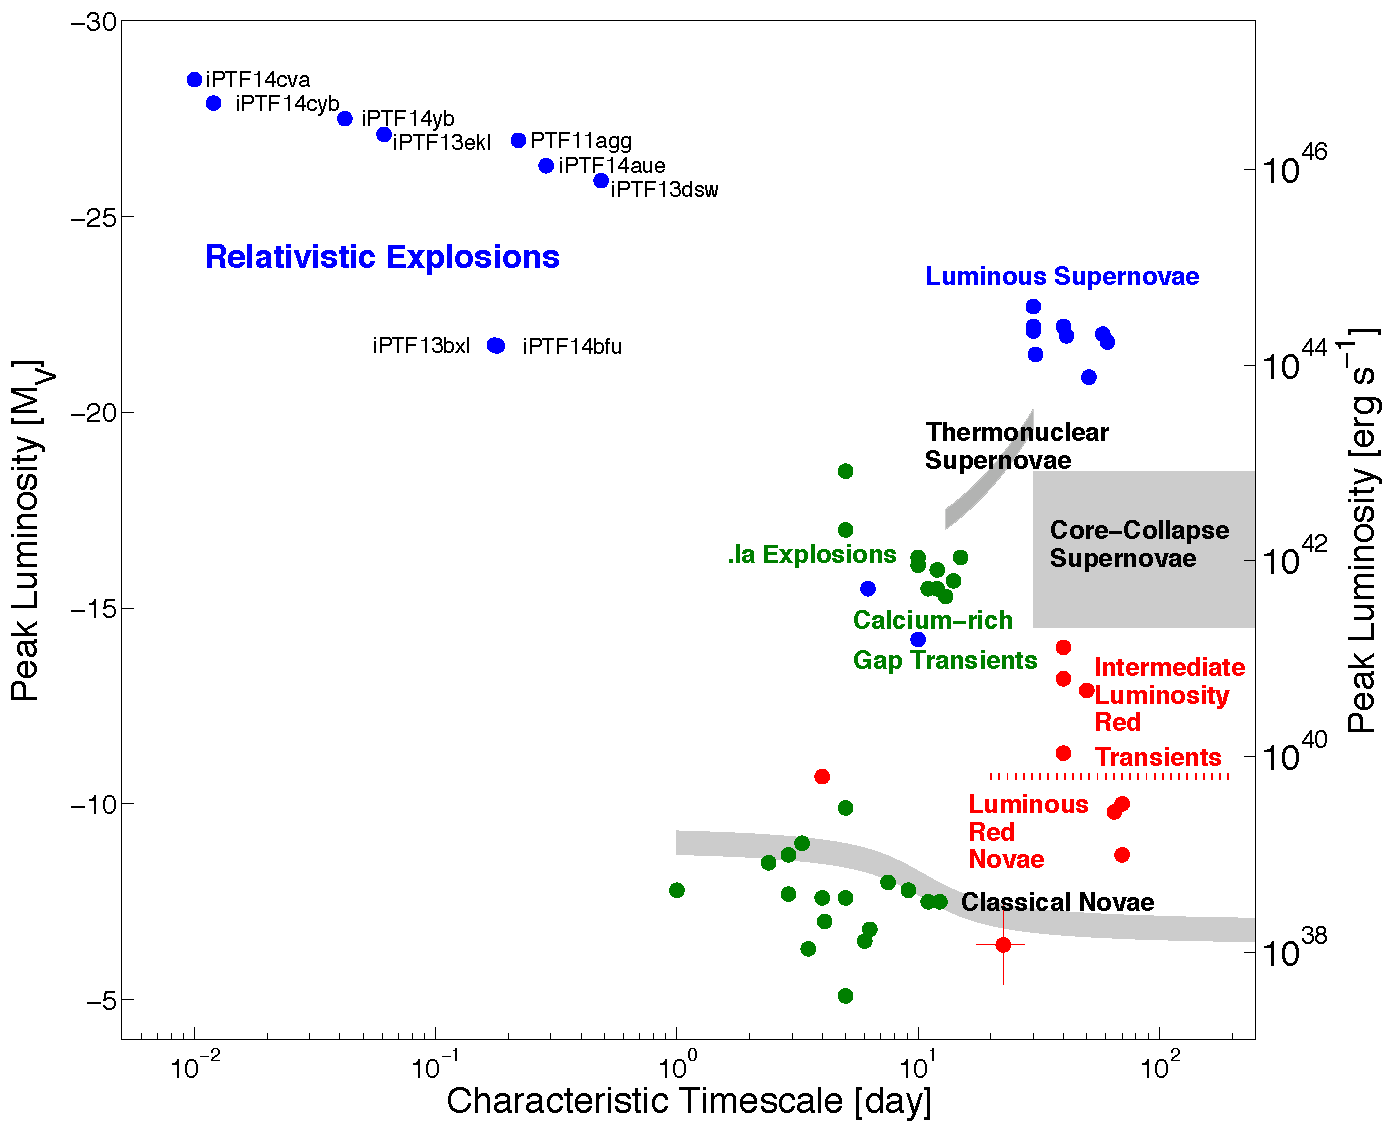
\includegraphics[width=0.6\textwidth]{figs/transients/taumv_2014.pdf}
}
\caption{
Peak luminosity-characteristic decay timescale plot for explosive
transients \citep[adapted from][]{2011PhDT........35K}.
}
\label{fig:transient_phase_space}
\end{figure}



%templates and stacks

%confusion

%


% --------------------------------------------------------------------


\subsection{Transient time scales}

Optical transients display a wide range of intrinsic timescales
(\autoref{fig:transient_phase_space}), and even some long-lived events 
have short-duration features of interest.

For very short-lived phenomena (stellar flares, GRBs),
the main function of LSST will be to provide discoveries and/or simple
characterization.  Followup to discovery/identification, if required,
must take place elsewhere. This implies that the LSST observations
must be sufficient to recognize in real time that an event is fast-evolving 
in order to to trigger followup. However, assessing the rise
slope is best done with a single filter, so prompt characterization
also needs multiple epochs within a night, preferably separated by at
least a few hours, in the same filter (we discuss this in detail in
\autoref{sec:\chpname:transientsAge}). That is, when observing with different
filters it is very difficult to separate lightcurve evolution from
color variations. Colors are informative when considering a statistical
samples (\autoref{sec:\chpname:SNtransients}): as long as the epoch of peak is
reliably assessed, coadded light curves and color time series can be studied.

SNe fall in an intermediate time range.  LSST will provide
multiple visits in multiple filters during the typical SN duration
(months).  This sampling may still be insufficient for many science
objectives, such as photometric classification of SN subtypes.
However, moderate changes to LSST
observing strategy may enhance the sampling for part of the sky part
of the time, greatly improving the usefulness of SN observations.
Metrics that assess the discovery rate of SN are included in
\autoref{chp:cosmo}.
Here we are interested in assessing the ability of
LSST to discriminate SN from other transients, SN subtypes from one
another, and to identify particularly interesting SNe: for example
those that show signature of shock break-out, or companion interaction
in the early light curve, and would be candidates for \emph{flash
spectroscopy} follow-up \citep[e.g.,][]{2014Natur.509..471G}.
In addition, metrics that
quantify LSST's ability to constrain SN physics in a statistically
large sample of SN are needed.

TDEs have only recently started to be characterized in the optical
bands. The current sample of events show relatively long
time-scales (rise and decline of the light curve is over months). We
would like to asses - through metrics - how well TDEs can be
distinguished from supernovae based on their light curve shape and
color (in real-time so that followup observations can be triggered)
and how well the LSST light curves themselves can be used to model the
TDE emission and deduce the black hole properties.
%Ref. Science Book:
%10.6.1, \citet{Gezari2012, Chornock2014, Arcavi2014, Holoien2014,
%Holoien2015, Holoien2016}.

Large amplitude flares from AGN may mimic
explosive transients; they are discussed in \autoref{chp:agn}.

In addition we hope that LSST will provide a wealth of serendipitous
discoveries of yet-to-be-observed transients.  An ideal transient
discovery survey would include balanced coverage of all time scales. LSST
will cover longer time periods well, but will have to make some
choices of emphasis in coverage of shorter time-scales.

In the sections that follow we will use several case studies to assess
LSST's performance for a range of time-domain science:

\begin{itemize}
\item
  The ability of a given LSST cadence to discriminate truly young
  transients from those only first detected well after their explosion date (\autoref{sec:\chpname:transientsAge}).
  This ability is a crucial input to follow-up strategy design.
  We identify a region of lightcurve slope
  % the phase-space of rising speed and color
  that is characteristic of a
  variety of transients in their early phases and assess the ability of LSST's
  cadences to place transients within this phase-space.
  More sophisticated classification algorithms will likely be necessary, but
  are beyond the scope of this whitepaper.
\item
  The statistical constraints to a transient class that can be obtained
  over the course of the LSST survey, from the LSST survey data alone
  (assuming a successful classification). SN Ia early interaction
  signatures or IIb shock break-out (\autoref{sec:\chpname:SNtransients}).
\item
  The ability to identify in real-time a rapidly-evolving
  object of interest and
  trigger prompt follow-up observations. For this topic GRBs are used as
  a case study (\autoref{sec:\chpname:grbs}).
\item
  The value of triggered Target-of-Opportunity observations for
  following up very rare, fast-evolving events.   Here the kilonova
  counterparts expected from Advanced LIGO triggers are used as a
  case study (\autoref{sec:\chpname:gw}).
\item
  The insight that a cadence gives into single transient classes. We
  discuss CVs, massive star eruptions, and TDEs (\autoref{sec:\chpname:future}).

\end{itemize}


% --------------------------------------------------------------------

\subsection{Metrics}
\label{sec:\chpname:metrics}

Two metrics were developed and are used in this chapter specifically for transient phenomena:
\begin{itemize}
  \item{\texttt{transientAsciiMetric}: accepts an ASCII file in input, so that realistic transient shapes can be used, with different shapes for different filters. The output can be the series of LSST observations (magnitude and error), or the fraction of transients detected (with user-specified constraints). This metric is used in \autoref{sec:\chpname:SNtransients}.}
  \item{\texttt{GRBTransientMetric}: caluclates the fraction of GRB-like transients detected (with user-specified constraints) using an $F(t) \propto t^{-\alpha}$
    lightcurve. This metric is used in \autoref{sec:\chpname:grbs}}.
\end{itemize}

Additionally, the standard MAF metrics 
that quantify the gaps between consecutive visits to
a field within a night and over multiple nights 
(\texttt{IntraNightGapsMetric} and \texttt{InterNightGapsMetric}) 
are of great value and are
heavily used throughout this chapter, in \autoref{sec:\chpname:transientsAge},
~\autoref{sec:\chpname:SNtransients}, and~\autoref{sec:\chpname:gw} for example.

Further metrics relevant to transient science are discused in \autoref{chp:galaxy},~\autoref{chp:cosmo}, and ~\autoref{chp:variables}. 

Many science cases can be developed and tested with these metrics, and we
encourage users to do so. In addition, we are collecting a library of representative transient lightcurves in a separate GitHub repository\footnote{\url{https://github.com/LSSTTVS/LSST_TVS_RoadMap}} and we encourage readers to contribute their transient models or observations.


% --------------------------------------------------------------------

\subsection{OpSim Analysis}
\label{sec:\chpname:analysis}

The current set of simulated cadences
provide poor coverage in any one
filter for transient events longer than a visit pair ($\sim$30
minutes) and shorter than $\sim$ weeks (\autoref{fig:tgaps} and 
\autoref{fig:tgaps_r}; \autoref{tab:visitgaps}).

As discussed in the subsequent sections, this
gap in the sampling hinders characterization of fast-evolving
transients.  A cadence with two visits separated by an hour or two rather
than 20 minutes would provide better discrimination.  A third visit in the
same night in a different filter would provide
color information valuable for realtime classification.
If a subset of those third
visits were in the same filter as the first two, it would improve the shape
characterization of the fastest-evolving transients.

\begin{table}
  \begin{tabular}{l|p{6cm}|c|c|c|c|p{5cm}}
    FoM & Brief description & {\rotatebox{90}{\opsimdbref{db:baseCadence}}}
          & {\rotatebox{90}{\opsimdbref{db:NEOswithVisitTriplets}}} &
          {\rotatebox{90}{\opsimdbref{db:NoVisitPairs}}} &
          {\rotatebox{90}{\opsimdbref{db:opstwoPS}}} & Notes \\
    \hline

    \thesection-1 & \footnotesize{\texttt{IntraNightGapsMetric},
    any filter}      & 0.39 & 0.42 & 0.18 & 0.40 &
    \footnotesize{Median gap (hours) between consecutive observations of a field
	    in any pair
    of filters in a single night.} \\

    \thesection-2 & \footnotesize{\texttt{IntraNightGapsMetric},
    $r$ band}      & 0.40 & 0.44 & 0.17 & 0.41 &
    \footnotesize{Median gap (hours) between consecutive $r$-band observations of a
	    field in a single night.} \\

    \thesection-3 & \footnotesize{\texttt{InterNightGapsMetric},
    any filter}      & 3.0 & 3.9 & 2.0 & 3.0 &
	    \footnotesize{Median gap (days) between consecutive observations of a field
	    in any pair
    of filters over multiple nights.} \\

    \thesection-4 & \footnotesize{\texttt{InterNightGapsMetric},
    $r$ band}      & 15.0 & 22.8 & 11.0 & 21.9 &
    \footnotesize{Median gap (days) between consecutive $r$-band observations
    of a field over multiple nights.} \\

\end{tabular}
\caption{
Inter- and intra-night revisit metrics in any filter and in $r$-band for
several simulated surveys.
}
\label{tab:visitgaps}
\end{table}

\begin{figure}[hbt]
\centerline{
	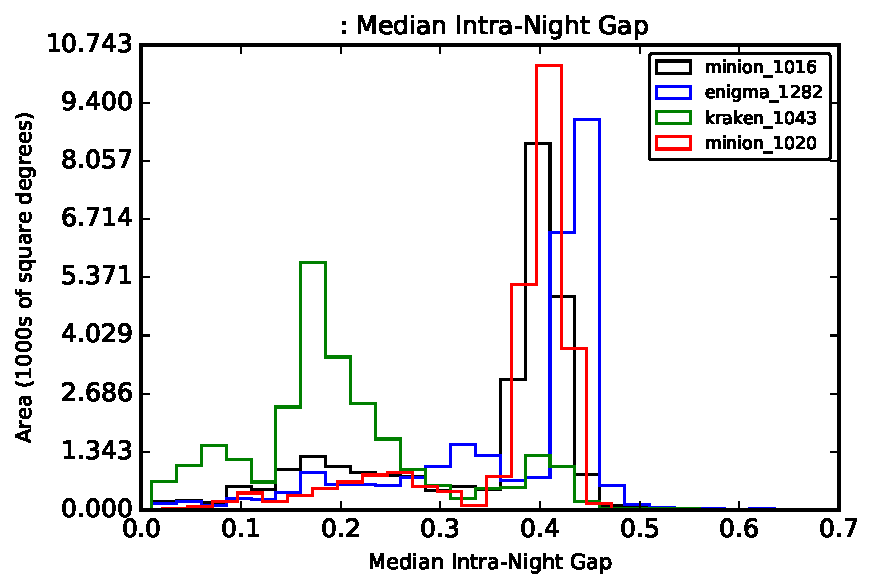
\includegraphics[width=0.45\textwidth]{figs/transients/MedianIntra-NightGap.pdf}
	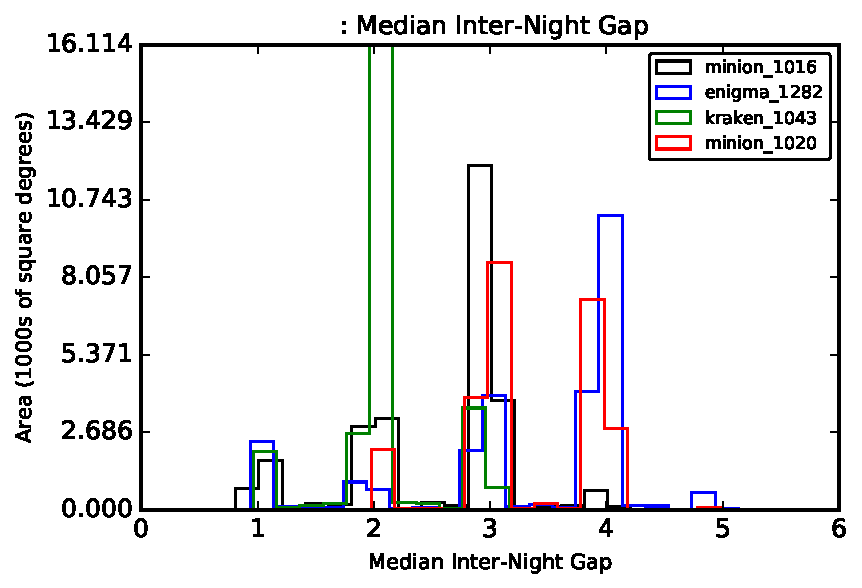
\includegraphics[width=0.45\textwidth]{figs/transients/MedianInter-NightGap.pdf}
}
\caption{ Histograms of median intra- (left) and inter- (right)
night visit gaps for any band for several OpSim runs. }
\label{fig:tgaps}
\end{figure}

\begin{figure}[hbt]
\centerline{
	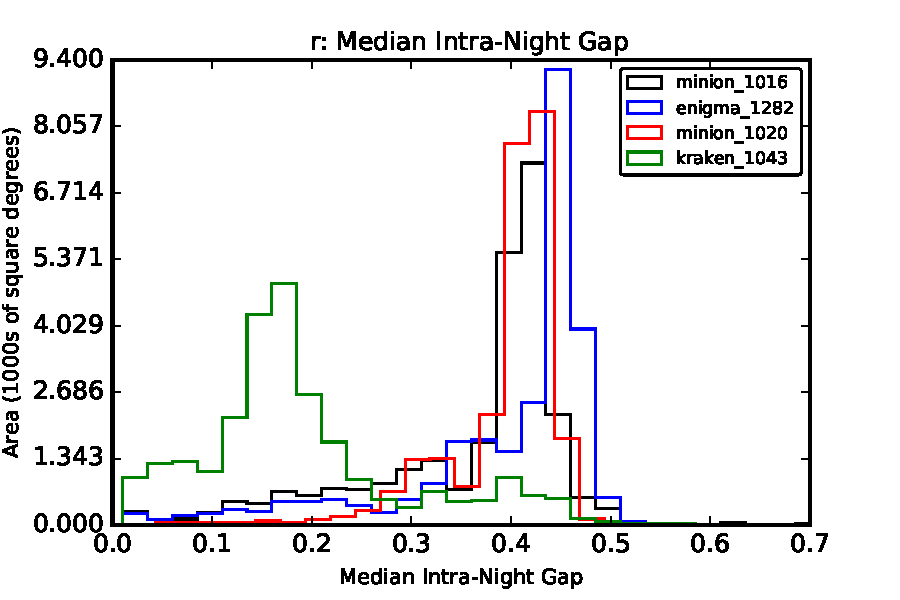
\includegraphics[width=0.45\textwidth]{figs/transients/MedianIntra-NightGap_r.pdf}
	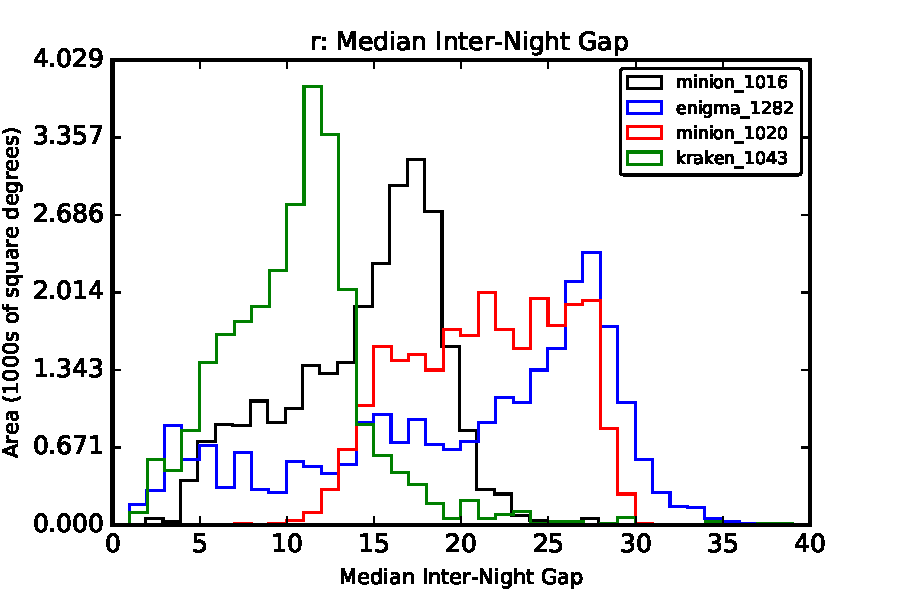
\includegraphics[width=0.45\textwidth]{figs/transients/MedianInter-NightGap_r.pdf}
}
\caption{ Histograms of median $r$-band intra- (left) and inter- (right)
night visit gaps for several OpSim runs. }
\label{fig:tgaps_r}
\end{figure}

% don't just care about gap between consecutive obs, though; first-last obs
% in a night
\emph{In fact, if the transient community were to design an optimal strategy for short and intermediate duration transients it would likely include 2 visits at a short time interval in different filter, and a third visit at a later time, but within the same night, with one of the two filters already used.}



% --------------------------------------------------------------------

\subsection{Discussion}
\label{sec:\chpname:discussion}

LSST's currently simulated cadences have significant cadence gaps for
timescales between nightly visit pairs and intra-night revisits.  For
many transient science cases, rolling-type cadences that improve the
sampling of a subset of events may be helpful in maximizing the
transient science that can be done with LSST: the minimum lightcurve
sampling required to adequately discover or characterize them may
still be larger than that provided by baseline cadences.  However,
even moderate adjustments (e.g., lengthening the visit pair spacing,
or optimizing the deep drilling filter strategy) may yield
improvements.  


The metrics presented in these sections are initial efforts towards
quantifying these goals, and they suggest specific directions for new
OpSIM experiments.  More detailed efforts to understand and model the
challenging problem of transient classification with sparse
lightcurves will be needed in order to best guide LSST's time-domain
observing strategy.


% --------------------------------------------------------------------

% ====================================================================
%+
% SECTION:
%    sn.tex  
%
% CHAPTER:
%    transients.tex  
%
% ELEVATOR PITCH:
%    Explain in a few sentences what the relevant discovery or
%    measurement is going to be discussed, and what will be important
%    about it. This is for the browsing reader to get a quick feel
%    for what this section is about.
%
% COMMENTS:
% ====================================================================
%+
% SECTION:
%    sn.tex  
%
% CHAPTER:
%    transients.tex  
%
% ELEVATOR PITCH:
%    Explain in a few sentences what the relevant discovery or
%    measurement is going to be discussed, and what will be important
%    about it. This is for the browsing reader to get a quick feel
%    for what this section is about.
%
% COMMENTS:
%
%
% BUGS:
%
%
% AUTHORS:
%  Stefano Valenti , Federica Bianco (@fedhere)
%
% ====================================================================

\section{Young Transients Discrimination Power}
\def\secname{transientsAge}\label{sec:\secname} % For example, replace "keyword" with "lenstimedelays"

\credit{svalenti} % (Writing team)

In this section we investigate the possibility to identify young transients using the intra-night visits. The Baseline Cadence predicts that on average, fields in the main survey get revisited about every 3 days using all filters, and every 15 days when using only r band visits (see section 2.2).  This means that we are likely to discover transients that are between 0 and 3 days old. As pointed out in section 6.1.2, the first hours after the explosion reveal fundamental information on the nature of transients. It is then important to be able to select, among the large number of transients discovered by LSST, the youngest objects. The Baseline Cadence predicts that the second intra-night visit will occur between 30 minutes to 2 hours after the first visit.  The question we are trying to answer here is: Which intra-night gap will maximize the identification of young objects?
To answer this question, we have selected a set of transients with good photometric coverage in the first week after the the outburst/explosion (see left panel of Figure 1) and compute the light curve slope (mag/day) as a function of time (see right panel of Figure 1). In Figure 2,  we report the change in brightness between the first and the second visit for a set of different transients as function of phase from explosion. Despite the heterogeneity in light curves shapes most of the transients show a similar change in brightens on a short time scale. 
This confirms that early classification and identification of interesting transients in a short time scale is a major challenge. However, independently on the type of transient, young transients may be easier to identify with large time gap between visits (2 hours). In general, most of the transients have a large increase in brightness at early phase. 
If the second visit occurs only 30 minutes after the first visit, the change in brightness will be of the order of 1$\%$ or less independently on the type of transient or the time from the start of the outburst/explosion, (see left panel of Figure 2). If the second visit occurs 2 hours after the first visit, the change of brightness will be large enough to be detected for young transients ($\sim$ 5$\%$). 
It is also worth to notice that a larger gap (24 hours), while could help in identify young transients, does not help in identify the type of transient.  The identification of interesting transients, at early stage, can be achieved using supplementary information like historical information from previous visits or color information of the transients.
Finally, we want to stress that the quality of early multiwavelengh data available today is still limited; the sample of astronomical transients used here is not comprehensive and an uniform set of homogeneous data of different transients is still needed in order to further investigate the need of color information. 

\begin{figure}[hbt]
\centerline{
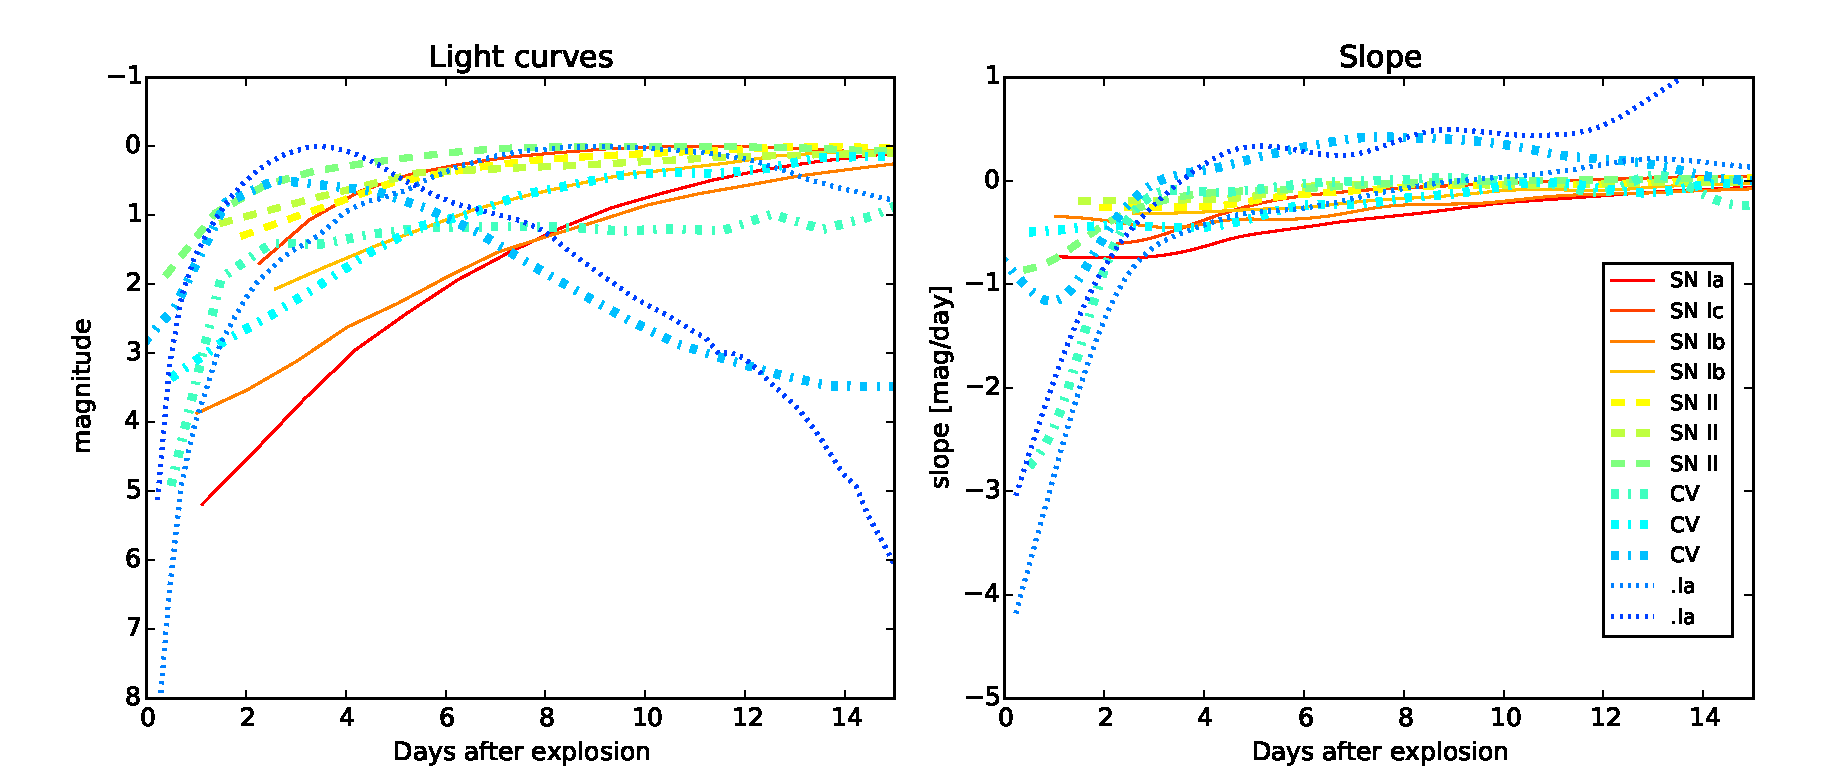
\includegraphics[width=0.6\textwidth]{figs/transients/earlyslope.pdf}
}
\caption{light curve slope [mag/days] of different type of transients as function of the phase from transient outburst/explosion.}
\label{fig:earlyslope}
\end{figure}

\begin{figure}[hbt]
\centerline{
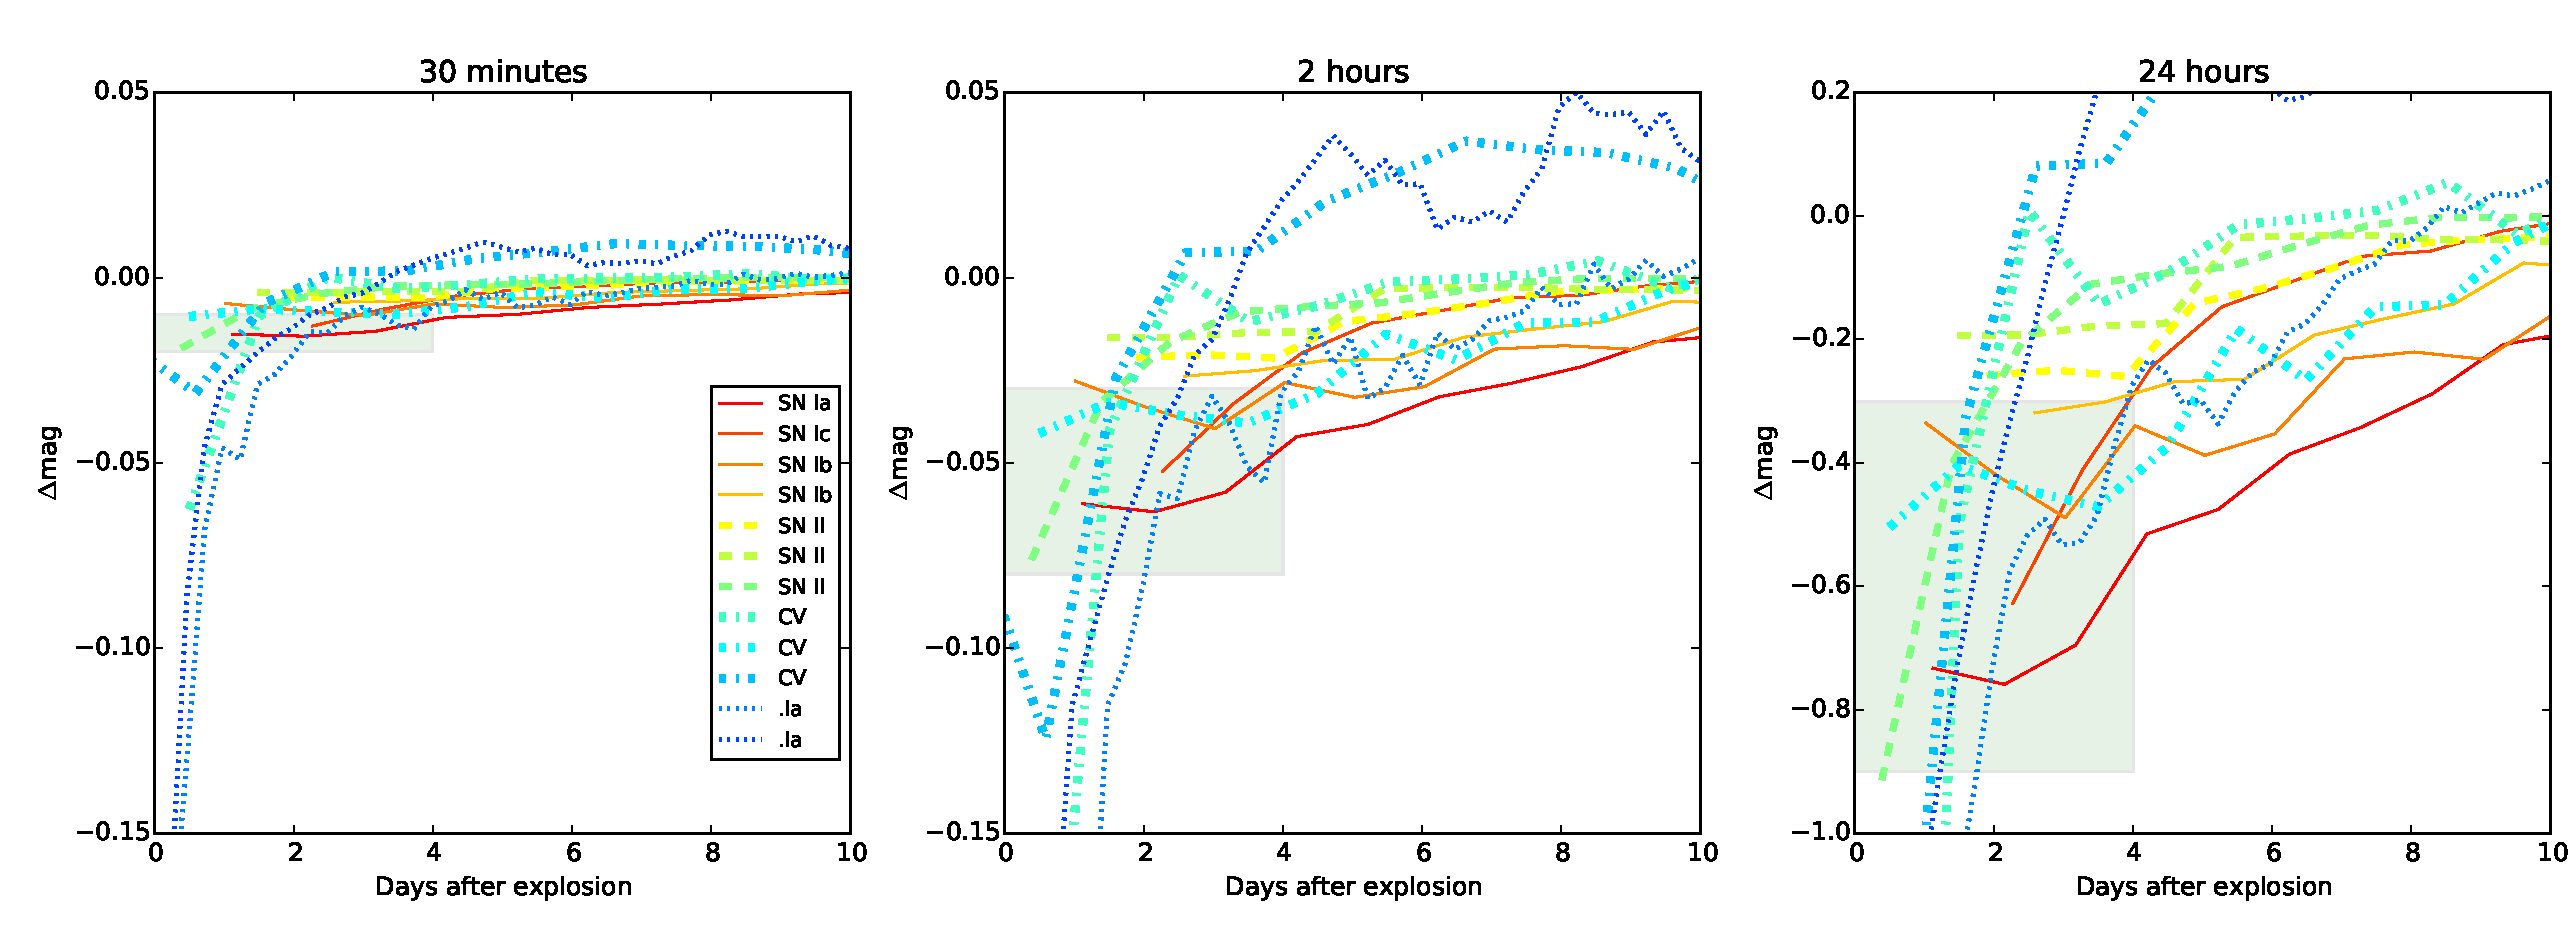
\includegraphics[width=0.6\textwidth]{figs/transients/earlyrise.pdf}
}
\caption{Expected difference magnitudes between two consecutive observations for a set of astronomical transients as a function of the phase of the transient. We consider the cases of the second observation occurring 30 minutes (left panel), 2 hours (central panel) and 24 hours (right panel) after the first observation. Data from: SN~Ia,  Olling et al 2015; SNII, Rubin et al 2016; SN~.Ia, 2010ApJ...715..767S; SN~Ib, Valenti et al 2011, Chao et al 2013; SN~Ic, Mazzali et al 2002; cv, Sokoloski et al. 2013, Finzell, et al in prep .
}
\label{fig:earlyrise}
\end{figure}
%%%%%%%%%%%%%%%%%%%%%%%%
%    Ineed to add the references
%
%Olling et al 2015, Nature, 521, 332O
%Rubin et al 2016, 2016ApJ, 820, 33R
%Valenti et al 2011, MNRAS, 416, 3138V
%Chao et al 2013,  ApJ, 775, 7C
%Mazzali et al, 2002, ApJ, 572L, 61M
%Sokoloski et al. 2013, 2013ApJ...770L..33S
%Finzell, et al in prep



% --------------------------------------------------------------------

% ====================================================================
%+
% SECTION:
%    sn.tex  
%
% CHAPTER:
%    transients.tex  
%
% ELEVATOR PITCH:
%    Explain in a few sentences what the relevant discovery or
%    measurement is going to be discussed, and what will be important
%    about it. This is for the browsing reader to get a quick feel
%    for what this section is about.
%
% COMMENTS:
%
%
% BUGS:
%
%
% AUTHORS:
%   Federica Bianco (@fedhere)
%
% ====================================================================

\section{Supernovae as transients}
\def\secname{SNtransients}\label{sec:\secname} % For example, replace "keyword" with "lenstimedelays"

\credit{fedhere} % (Writing team)

Supernovae (SNe) are the final dramatic stages of stellar life. SNe include a diverse set of phenomena: explosion of low mass stars in binary systems, thermonuclear SN or SN Ia (also discussed in \ref{sec:supernovae}), and explosion of high mass stars, Core collapse (CC) SNe. Phenomenologically the observable of the explosion are themselves diverse.  The transient duration ranges between weeks and months, possibly years. The electromagnetic energy radiated ranges between $\sim0.1$ (faintest CC SNe), to $\sim1$ (SN Ia) and $\sim100$ (Superluminous SNe, SLSNe) ($\times 10^{49}$ erg), corresponding to absolute magnitudes at peak ranging between $\sim-19$ and $\sim-22$.

LSST's contribution to SNe studies can can be substantial, on many different aspects. The first crucial input will be discovery: we expect as many as $\sim 1000$ SN discoveries per night. The first step is then \emph{discrimination}, and the first question we need to answer, with a metric, is: will LSST photometry allow to distinguish the different types of SN to appropriately direct follow-up efforts?

When a large statistical sample of SNe is generated, LSST's photometry may allow to set constraints on the diversity of the sample, and thus inference on the diversity within the population of SN, which in turn may constrain the genesis of the explosion. Outstanding questions that can be answered statistically are: what is the percentage of SN Ia that arise from a \emph{single degenerate} progenitor system (a CO WD-WD binary), from a {\emph single degenerate} system (a WD-MS or WD-RG binary), or a {\emph merger} (a WD-WD binary with a He and a CO WD) (citation). Answering this question may reduce the scatter in the Hubble diagram, if SNe from different progenitors are shown to require different standardization (citation). On the CC SN side: the diversity of SN subclasses, and the relationship between them (is there a phenomenological continuum or actually distinct classes, e.g. between IIp-IIL, IIb-Ib?) is yet to be understood. Individual well studied objects may answer these questions, for example individual SN Ia with tight constraints on the progenitor system show that both single and double degenerate progenitors exist (e.g. SN 2011fe, \citealt{Li2011}, and PTF 11kx, \citealt{Dilday11}). However, a statistical sample is suitable to set constraints on populations. Thus the question  we need to answer, with a metric, is: how much detail can be sacrificed in favor of sample size without compromising diagnostic power? And the diagnostic power relies on color and sampling: thus what is the trade-off between cadence in the same filter, and observations in different filters. Specifically, transients can be distinguished early from two photometric characteristics: rise time and color. There is a tension between these observables: obtaining colors relies of course on obtaining photometry in different bands at within short time scales, ideally simultaneously, although within a night is probably sufficiently close. However, assessing the rise slope is best done with a single filter, so prompt characterization also needs multiple epochs within a night, although separated by at least a few hours, in the same filter. That is: observing with differnt filters it is impossible (or very hard) to separate shape from color. Colors of course allow to learn a lot more about the statistical sample: as long as the epoch of peak is reliably assessed coadded lightcurves can be studeid (Bianco 2011).


Thus we envision 2 SN related metrics: 
\begin{itemize}
\item a metric that assess the ability of a cadence to distinguish between SNe among all transients, the ability to distinguish among SN subtypes, and within a subtype the ability to gauge how typical, or atypical (and thus worthy or particular attention) a SN is. 
\item a metric that works on a large sample (3-, 6-, 9-years of LSST data) and assess the ability to characterize the contribution of SN with specific features to the population: as a test case we will use the presence of an early blue excess for type Ia, signature of interaction with a companion, and the presence of an early blue escess signature of shock breakout for CC SNe.
\end{itemize}


% --------------------------------------------------------------------

% ====================================================================
%+
% SECTION:
%    grb.tex  % eg lenstimedelays.tex
%
% CHAPTER:
%    transients.tex  % eg cosmology.tex
%
% ELEVATOR PITCH:
%    Explain in a few sentences what the relevant discovery or
%    measurement is going to be discussed, and what will be important
%    about it. This is for the browsing reader to get a quick feel
%    for what this section is about.
%
% COMMENTS:
%
%
% BUGS:
%
%
% AUTHORS:
%    Phil Marshall (@drphilmarshall)  - put your name and GitHub username here!
%-
% ====================================================================

\section{Gamma-Ray Burst Afterglows}
\def\secname{grbs}\label{sec:\secname} % For example, replace "keyword" with "lenstimedelays"

\credit{ebellm} % (Writing team)

Gamma-ray bursts (GRBs) are relativistic explosions typically classified by the temporal duration of their initial gamma-ray emission: Long GRBs, that mark the endpoint of the lives of some massive stars, and short GRBs, believed to originate from the merger of binary neutron stars.
GRB emission is known to be beamed: the initial prompt gamma-ray emission is seen only for observers looking at the jet axis. The longer-wavelength X-ray, optical, and radio afterglow may be seen both by on- and off-axis observers.  The latter case is known as an orphan afterglow, due to the absence of gamma-ray emission.  
On- and off-axis afterglows are predicted to have different temporal signatures in the optical: On-axis events decay as a power-law until a jet break, while off-axis events should be fainter and show an initial rise 
Despite systematic searches, no convincing orphan afterglow candidates have yet been discovered, limiting our knowledge of the beaming fraction of GRBs and hence their true rates.
Well-sampled orphan afterglow lightcurves would also permit study of the GRB 
jet structure.

Because of their rarity, in all but one case \citep{2015ApJ...803L..24C} to date GRBs have been discovered using their prompt emission by hard X-ray or gamma-ray all-sky monitors.  
This selection imposes biases on the population of relativistic explosions we observe.  
Baryon-loading in the GRB jet---a ``dirty fireball'' \citep{2003ApJ...591.1097R}---can lead to on-axis events without gamma-ray emission.  Only one plausible candidate has been identified to date \citep{2013ApJ...769..130C}.  
Discovery of new dirty fireballs---if distinguished from off-axis events--would clarify the rates of these events and enhance our understanding of the diversity of stellar death.

LSST is the survey most capable of resolving these decades-old questions.  Due to its large aperture and etendue, LSST can detect faint, fast-fading, and rare cosmological events, potentially enabling population studies of the high-redshift universe.  
\citet{2015A&A...578A..71G} estimated LSST could detect 50 orphan afterglows each year, more than any other planned survey.

%deep survey helps due to time dilation

%beaming fraction and true rates; jet structure; dirty fireballs?
%GRB-SN connection; probe high-z star formation?

%other fast transients: Fast transients and SN shock breakout?  flash spectroscopy

% --------------------------------------------------------------------

\subsection{Target measurements and discoveries}
\label{sec:\secname:targets}

GRB afterglow discovery is among the science cases that places the greatest stress on the LSST cadence.  Because afterglows fade rapidly---dropping several magnitudes in the first few hours---high cadence observations are required to detect the fast fading.  
If an afterglow candidate can be recognized in real time, it will be possible to trigger TOO spectroscopy (to measure a redshift and confirm the event is cosmological), X-ray observations (to detect a high-energy counterpart), and additional photometry (to characterize the lightcurve evolution).  If there is no source at the location of the transient in the coadded reference image, two consecutive observations in the same filter separated by an hour or two are the minimum required to potentially trigger followup of a fast-fading event.  
However, a third or fourth observation in a single night---ideally in the same filter---would improve the purity of the sample.  Observations in other bands at high cadence are less useful because they require assumptions about the event's SED and its evolution to determine if a source is truly fading.

Distinguishing orphan afterglows from on-axis events (whether conventional GRBs or dirty fireballs) will also require more than two detections.  Orphan events may prove harder to recognize in real time, because they are intrinsically fainter than on-axis events and show an initial rise rather than a rapid decay.  
Additionally, because of relativistic time dilation high redshift events are easier to detect, but these events will be fainter and more difficult to follow up.
Accordingly, population studies of orphan afterglow candidates may be best conducted with LSST photometry alone.  These may only be productive if LSST has suffiently frequent revisits to a field in a single filter.


% --------------------------------------------------------------------

\subsection{Metrics}
\label{sec:\secname:metrics}

The core figure of merit for GRB afterglows is simply the raw number of on- and off-axis events detectable in two, three, or more observations, preferably in a single filter.

The appropriate way to derive these detections is to conduct a Monte Carlo simulation of a cosmological population of GRBs and fold it through the LSST observing cadence \citep[cf.][]{2011PASP..123.1034J}.  We are pursuing developing this infrastructure in the MAF framework.  

Simplified metrics can give us a general idea of how well a given cadence can characterize fast-evolving transients such as GRBs.


% --------------------------------------------------------------------

\subsection{OpSim Analysis}
\label{sec:\secname:analysis}

OpSim analysis: how good would the default observing strategy be, at
the time of writing for this science project?


% --------------------------------------------------------------------

\subsection{Discussion}
\label{sec:\secname:discussion}

Discussion: what risks have been identified? What suggestions could be
made to improve this science project's figure of merit, and mitigate
the identified risks?


% ====================================================================

\navigationbar


% --------------------------------------------------------------------

% PJM: moved to Future Work while MAF analysis is pending:
% % ====================================================================
%+
% SECTION:
%    tde.tex
%
% CHAPTER:
%    transients.tex
%
% ELEVATOR PITCH:
%    Tidal disruption events (TDEs) are the disruptions of stars by supermassive black holes.
%    They can produce flares in the optical and UV (sometimes accompanied by X-ray and radio emission as well).
%    These flares can be used to reveal the properties of otherwise quiescent SMBHs and to study accretion physics.
%    TDEs are rare, LSST will allow the first statistical sample of such events.
%
% AUTHORS:
%    Iair Arcavi (@arcavi)
%
% ====================================================================

% \section{Tidal Disruption Events}
\subsection{Tidal Disruption Events}
\def\secname{\chpname:tdes}\label{sec:\secname}

\credit{arcavi}

A star passing close to a supermassive black hole (SMBH;
$M\gtrsim10^{6}M_{\odot}$) will be torn apart by tidal forces. For
certain ($\lesssim10^{8}M_{\odot}$) black hole masses, the disruption
will occur outside the event horizon and will be accompanied by an
observable flare \citep{Hills1975, Rees1988}. Such flares can be used to
study inactive SMBHs, which are otherwise inaccessible beyond the nearby
($\lesssim100$ Mpc) universe.

We are now building our understanding of how observational properties of
TDEs are affected by the SMBH. Theory claims to provide such a
connection \citep[e.g.][]{Lodato2009, Guillochon2014}, but uncertainties
in the physics of the disruption, subsequent accretion and emission
mechanisms are currently topics of debate \citep[e.g.][]{Strubbe2015,
Guillochon2014, Roth2015}, and new models are vigorously being developed
\citep[e.g.][]{Piran2015, Hayasaki2015, Svirski2015, Bonnerot2015}.

TDEs are rare ($\sim10^{-5}-10^{-4}$ events per galaxy per year;
\citealp{Wang2004, Stone2015}), and until recently, TDE candidates were
discovered mostly in archival data \citep[e.g.][]{Donley2002,
Gezari2006, Esquej2007}. Now, however, wide-field transient surveys have
started discovering TDEs in real time.

Generally, two types of TDE candidates have been identified:
\begin{enumerate}
\item High energy TDEs - The prototype of which is Swift J1644
\citep{Bloom2011, Burrows2011, Levan2011, Zauderer2011}, with two other
events known \citep{Cenko2012, Brown2015}. These events display emission
in $\gamma$-rays and X-rays as well as in the radio, but are not
detected in the optical.
\item Optical-UV TDEs - The prototype of which is PS1-10jh
\citep{Gezari2012}. About $8$ other events are known
\citep{Chornock2014, Arcavi2014, Holoien2014, Holoien2015, Holoien2016}.
Some events were detected also in the X-rays and radio (in addition to
the optical and UV), but the X-ray and radio signatures are different
than those of the high energy TDE candidates.
\end{enumerate}

It is still not clear whether both of these classes of transients are TDEs,
and if so, why they are so different form each other. One option raised is
that some TDEs may launch jets, which when directed towards us, appear as
the high energy events, but otherwise appear as the optical-UV events.
It is still not clear if this is indeed the case \citep[e.g.][]{VanVelzen2013}.

Here we focus on the second type of TDE candidates, which is the
relevant class for LSST, since they can be discovered in the optical.
However, multi-wavelength coordinated observations of
optically-discovered events are required in order to better understand
the connection between the two types of candidates.

The first well-sampled TDE of the optical+UV class was PS1-10jh (discovered by Pan-STARRS;
\citealt{Gezari2012}). \citet{Arcavi2014} later presented three new TDE candidates
from PTF and one discovered by ASAS-SN, all with similar properties
as PS1-10jh. These events exhibit blue colors, broad light curves,
peak absolute magnitudes of $\sim-20$ and a $\sim t^{-5/3}$ decay
at late times. This decay law has been suggested as a unique signature
of accretion-powered TDE light curves \citep{Rees1988, Evans1989, Phinney1989}.
Early-time deviations from the $t^{-5/3}$ rate
can be used to constrain the density profile of the disrupted star
\citep{Lodato2009, Gezari2012}. Late-time deviations would
test the accretion power-source hypothesis altogether.

The spectral signatures of these TDEs are still a puzzle. PS1-10jh displayed
only He II emission lines, lacking any signs of H. Some of the \citet{Arcavi2014}
sample, however, do display H emission.
In fact, a continuum of H / He emission ratios for this class of transients
is being revealed, and is now a focus of theoretical modelling \citep{Strubbe2015, Roth2015}.

The second recent discovery relating to this new sample concerns their
host galaxies \citep{Arcavi2014, French2016}, most of which are
post-starburst galaxies. These galaxies show little or no signs of on-going star formation, but their significant A stellar populations indicate that star formation ceased abruptly a few hundred Myr to a Gyr ago \citep{Dressler1983}. Galaxies with these characteristics often show signs of recent galaxy-galaxy mergers \citep{Zabludoff1996}, which produced the starburst and evolved the bulge. Optical-UV TDEs are intrinsically over abundant in post-starburst galaxies by a factor of $\sim30-200$ (depending on the characteristics of the galaxy; \citealt{French2016}). The reason for the strong preference of TDEs for post-starburst galaxies has still not been determined.

LSST's contribution to TDE studies will be substantial.
\citet{VanVelzen2011} estimate that LSST could discover approximately
4000 TDEs per year. The main drivers for studying TDEs with LSST are:
\begin{itemize}
\item Measuring black hole masses: This involves fitting models to TDE
light curves. It is also relevant to correlate these measurements with
host galaxy properties (mass, bulge/disk decomposition).
\item Constraining galactic dynamics by measuring the TDE rates as
functions of black hole mass and galaxy types.
\item Characterizing TDE emission signatures.
\end{itemize}

A metric is required for measuring how well TDEs can be identified and
distinguished from supernovae and active galactic nuclei. In general, we
expect TDEs to:
\begin{itemize}
\item Be located in the center of their host.
\item Display approximately constant blue (few $10^4$K) colors.
\item Evolve slowly (weeks-months).
\item Not show past AGN-like variability.
\item Preferentially peak around mag -20.
\item Preferentially be hosted in a post-starburst galaxy.
\end{itemize}
These criteria are based on our current knowledge of optical TDEs, which
is still in its early stages. The field is rapidly evolving, and it is
possible that new observations will change the current picture of TDE
emission. This metric is probably best combined with those discussed in
 \autoref{sec:\chpname:SNtransients} for identifying supernovae, though the
luminosity function of TDEs (or what constitutes a ``typical'' TDE light
curve) is not yet known.

A second metric is required to asses the accuracy with which the black
hole mass can be constrained from the TDE light curves. This metric can
be based on existing theoretical models to fit simulated TDE light
curves (such as TDEFit; \citealt{Guillochon2014}).


% --------------------------------------------------------------------

% PJM: moved to Future Work while MAF analysis is pending:
% % ====================================================================
%+
% SECTION:
%    sn.tex  
%
% CHAPTER:
%    transients.tex  
%
% ELEVATOR PITCH:
%    Explain in a few sentences what the relevant discovery or
%    measurement is going to be discussed, and what will be important
%    about it. This is for the browsing reader to get a quick feel
%    for what this section is about.
%
% COMMENTS:
%
%
% BUGS:
%
%
% AUTHORS:
%   Federica Bianco (@fedhere)
%
% ====================================================================

\section{Cataclismic Variables}
\def\secname{CVtransients}\label{sec:\secname} % For example, replace "keyword" with "lenstimedelays"

\credit{paulaszkody}, \credit{fedhere} % (Writing team)

Cataclysmic Variables (CVs) encompass a broad group of objects
including novae, dwarf novae, novalikes, and AM CVn systems, all with different
amplitudes and rate of variability. The one thing they all have in
common is active mass transfer from a late type companion to a
white dwarf. The variability ranges from minutes (due to the flickering in
dwarf novae and novalikes, the pulsations in accreting white dwarfs in
the instability strip, or the orbital periods of AM CVn systems), to
hours (for the orbital periods of novae, dwarf novae and novalikes) to
days (for the normal outburst lengths of dwarf novae) to 
weeks (for the outburst length of superoutbursts in short orbital period
dwarf novae and the outburst recurrence time of normal outbursts in short
orbital period dwarf novae) to months (for the outburst recurrence time of 
longer period dwarf novae, various state changes in novalikes and the decline 
in novae) and, finally, to years (for the outburst recurrence timescales of the 
shortest period dwarf novae and the recurrence times in recurrent novae). The 
amplitudes range from tenths of mags for flickering and pulsations to 4 mags 
for normal dwarf novae and changes in novalike states up to 9-15 mags for the 
largest amplitude dwarf novae and regular novae.

These large differences make correct classification with LSST difficult
but necessary in order to reach goals of assessing the correct number
of types of objects for population studies of the end points of
binary evolution. Multiple filters (especially the blue $u$ and $g$) 
along with amplitude and recurrence of variation provide the best
discrimination, as all CVs are bluer during outburst and high states of
accretion. Long term evenly sampled observations can provide indications
of the low amplitude random variability and catch some of the more frequent
outbursts but higher sampling is needed to determine whether an object
has a normal or superoutburst, to catch a rise to outburst or to a
different accretion state or to follow a nova. Novae typically
have rise times of a few days while the decline time and shape provide
information as to the mass, distance and composition. The time to decline
by 2-3 magnitudes is correlated with composition,

***FED: what is a range of time scales for this decline? days? months?

WD mass and location in
the galaxy, thus enabling a study of Galactic chemical evolution.  As with SN, 
the diagnostic power for all these systems rests on color and sampling.   

The metrics rely on a given cadence to provide shape and recurrence time
of large variations that will distinguish between new novae, dwarf novae
outbursts and identify hig vs low states, as well as available blue colors to 
distinguish low amplitude variability that would indicate new pulsators or 
novalikes. The population studies rely on the numbers of long orbital period 
(low amplitude, wide outbursts) vs short orbital period (patterns of short 
outbursts followed by larger, longer superoutbursts) dwarf novae at different 
places in the galaxy, as well as the numbers of recurrent (1-10 yrs) vs normal 
novae (10,000 yrs, about 35/galaxy/yr). Objects particulary worthy of 
discrimination for later followup are the numbers of CVs containing highly 
magnetic white dwarfs. These can be identified by a metric of 10 yrs of data on
a large sample where the magnitude for a majority of the years is a faint (low)
state and a small percentage of time is a bright (high) state, combined with a 
red color (due to cyclotron emission from the magnetic accretion column).


% --------------------------------------------------------------------

% PJM: moved to Future Work while MAF analysis is pending:
% % ====================================================================
%+
% SECTION:
%    eruptive.tex
%
% CHAPTER:
%    transients.tex
%
% ELEVATOR PITCH:
%-
% ====================================================================

% \section{LBVs and related non-supernova transients}
\subsection{LBVs and related non-supernova transients}
\def\secname{\chpname:LBVs}\label{sec:\secname}

\credit{nathansmith}

There is a large and diverse class of visible-wavelength transient
sources recognized in nearby galaxies that appear to be distinct from
traditional novae and from SNe, and have often been associated with
the giant eruptions of luminous blue varibles (LBV), such as the 19th
century outburst of $\eta$ Carinae.  Broadly speaking, members of this
class of transients share the common properties that they have peak
luminosities below those of most core-collapse SNe and more luminous
than novae and CVs (absolute magnitudes of roughly $-$9 to $-$15 mag).
They also have H-rich spectra (usually) with relatively narrow lines
that indicate modest bulk outflow velocities of 10$^2$ to 10$^3$ km
s$^{-1}$ (although some have exhibited small amounts of material at
faster speeds).  They tend to evolve on fairly long timescales of
weeks to years (although sometimes they exhibit a quick rise to peak
similar to SNe II-P). This group of transients has gone by many names,
such as LBV eruptions, SN impostors, Type V supernovae,
intermediate-luminosity optical (or red) transients, as well as others
that often include a physical interpretation.  For brevity, these are
often collectively referred to as ``LBVs'', although many of them may
not actually be LBVs.
%This may be largely for historical reasons,
%since LBVs were the first of these to be recognized as a class.  Some
%of the subgroups may be very different from objects like $\eta$
Carinae, however.

Observationally, these eruptions are understood to represent important
and dramatic mass-loss episodes in the lives of massive stars, based
on empirical estimates for the amount of ejected matter.
%Guided
%largely by nearby LBVs with resolved shells, t
These eruptions are
expected to instigate mass loss that is comparable to or more
important than metallicity-dependent winds of massive stars.  This
mode of mass loss, regardless of the mechanism, may be a very
important ingredient in the evolution of massive stars that is
currently not included in stellar evolution models.  Correcting this
is one of the key science drivers in trying to understand the physics
these eruptions.

An important empirical discriminant of subgroups in this class comes
from their progenitor stars.  Some are indeed seen to be very
luminous, blue supergiant stars consistent with traditional LBVs.
Some, however, have somewhat less luminous, heavily dust-obscured
progenitor stars that have been associated with either dust enshrouded
blue or red supergiants, or alternatively, with super-AGB stars of
8-10 M$_{\odot}$, with uncertainty .
%The degeneracy
arises because when the objects are
fully obscured by dust, one cannot actually meaure the star's
temperature, and the bolometric luminosities of super-AGB and red and blue supergiants overlap.  Unfortunately,
cases when we have strong constraints on the quiescent progenitor are
rare, and once they reach their peak luminosity, there is a great deal
of overlap in observed properties.

Theoretically, these eruptions are not understood.  There are many
ideas, but few if any confirmed mechanisms tied to observed
objects.
Some
%previously discussed
theoretical ideas involve (1)
winds driven by super-Eddington instabilities (although the root cause
for suddenly exceeding the Eddington limit remains unexplained), (2)
hydrodynamic explosions caused by deep-seated energy deposition, such
as unsteady nuclear burning, (3) accretion onto companion stars in
binary systems (degenerate or not), (4) mergers in binary and triple
systems, (5) electron-capture SNe, and (6) ``failed SNe'' associated
with a weak explosion and envelope ejection that results from black
hole formation during core collapse.
Because of the relatively low total energy indicated by
radiative luminosities and outflow speeds, these are usually discussed
as non-terminal eruptions, however, the last two are terminal events
that are less luminous and lower energy than normal SNe, and the last
3 should only occur once for a given source.
Together with several well-studied examples that indicate
repeating eruptions, there are indeed many
cases where only one such transient has been seen at the same
position, and some cases where late-time observations suggest that no
source has survived with a luminosity comparable to its progenitor.
%However, there are also several well-studied examples that indicate
%repeating eruptions (multiple repeating transients, multiple nebular
%shells with different ages, etc).
All these theoretical mechanisms
may lead to similar observed phenomena: weak explosions, moderate
luminosities, slow expansion, dusty aftermath, but this class of objects
may represent a mixed-bag of different mechanisms that get lumped
together by default as ``other'' because they are not traditional SNe.

An area of recent interest
is that eruptive non-terminal transients have been observed, in some
cases, to precede much more powerful explosions that are seen as Type
IIn supernovae.  Detectability of SN precursors is discussed in ~\autoref{chp:galaxy}. Even if the pre-SN transients are not observed
directly, pre-SN eruptive mass loss is inferred based on circumstellar
interaction diagnistocs of the SN.  These SN precursors have observed
or inferred properties that are very similar to LBVs and related
transients, 
%.  This may suggest some link between them,
but then again,
most of the LBVs and other SN impostors have been observed for decades
and have not gone SN (yet).  \emph{Being able to distinguish which of these
optical transients are SN precursors and which are not is a major
science driver.}  The amount of mass lost in a precursor eruption may
dramatically alter the type of SN that is observed.  There may also be
a continuum of energies in pre-SN outbursts, extending down to more
normal classes of core-collapse SNe, but these may often go
unrecognized unless the SN is caught very early after explosion.

Rates for these LBV-like eruptions are very poorly constrained,
largely because most previous SN and transient searches with small
telescopes have been optimized for finding more luminous SNe in a
larger volume.  This field begun to change with recent surveys, and will
be revolutionized with LSST.  From discovered examples we have,
numbers are very roughly consistent with a volumetric rate comparable
to that of core-collapse SNe or larger.  %, but with a large error bar.
Rates of individual subclasses are not well constrainted, and limited
information often makes classification into various subgroups
difficult or highly subjective.  The ``rate'' also depends on how
faint the lower limit of inclusions is; evidence suggests that the
brightest events are more rare, and that numbers increase as one moves
to lower luminosity.  At the faint end, it becomes difficult to
distinguish between eruptions and regular variability of LBVs, or
between massive star eruptions and CVs. With deep LSST stacks identifying faint CV in quiescent states this will also change dramatically in the LSST age, with the unvailing of detailed progenitor
information.  Having deep, pre-eruption characterization
of sources at the positions of these eruptive transients (as well as
SN precursors) will likely be a major contribution of LSST.

In terms of timescales, many of the eruptive transients exhibit rise
and decline timescales similar to normal SNe~II-P or II-L, but with
fainter peak luminosity.  For these, observational cadence
requirements will be the same as SNe.  For some eruptive transients,
however, the rise timescales can be very long (rising a few magnitudes
in years).  While LSST's cadence will certainly be fast enough, being
able to discover slowly rising tranients that do not change much from
night to night will be an important metric.

For the faster-rising transients, spectroscopic followup is needed to
discriminate these from normal SNe, and also contextual information
about the host galaxy (and hence, the absolute magnitude) is needed to
differentiate these non-terminal eruptions from Type IIn supernovae
(their spectra look similar, although LBVs do tend to have narrower
lines).  Spectral and color evolution, as well as information about
the progenitor, is needed to distinguish among subgroups within the
class.  Multiwavelength followup is often extremely valuable or even
essential; i.e. mid-IR tells us if an optically invisible source is
cloaked in a dust shell but still quite luminous; Xrays and radio tell
us if an expanding shock wave is the likely source of persistent
luminosity.  For these reasons, nearby cases will continue to be the
most valuable in deciphering the physics of subclasses, whereas the
increased volume in which LSST discovers these fainter transients will
drastically improve our understanding of their rates.  Armed with both
a better understanding of their underlying physics and
characterization, as well as their rates and duty cycles, these
eruptive events can then be incorporated into stellar evolution models
and population synthesis/feedback models.

% % --------------------------------------------------------------------
%
% \subsection{Metrics}
% \label{sec:\secname:metrics}
%
% % --------------------------------------------------------------------
%
% \subsection{OpSim Analysis}
% \label{sec:\secname:analysis}
%
% % --------------------------------------------------------------------
%
% \subsection{Discussion}
% \label{sec:\secname:discussion}
%
% % ====================================================================
%
% \navigationbar


% --------------------------------------------------------------------

% ====================================================================
%+
% SECTION:
%    gw.tex
%
% CHAPTER:
%    transients.tex
%
% ELEVATOR PITCH:
%-
% ====================================================================

\section{Gravitational Wave Sources}
\def\secname{\chpname:gw}\label{sec:\secname}

\credit{raffaellamargutti},
\credit{Doctor},
\credit{Fong},
\credit{Haiman},
\credit{Kalogera},
\credit{Trimble},
\credit{Zauderer}

The first detection of Gravitational Waves (GW) by the advanced
LIGO/Virgo collaboration \citep{Abbott16, Abbott09, Acernese08} has
recently opened a new window of exploration into our Universe. The
amount of information that can be revealed by the properties of the GW
emission is immense and holds promises for revolutionary insights,
including accurate masses and spins of neutron stars and black holes,
tests of General Relativity and an accurate census of the neutron star
(NS) and black hole (BH) populations that might challenge our current
understanding of massive stellar evolution. However, GW events are
poorly localized (10-100 deg$^2$ at the time of LSST operations). The
identification of EM counterparts would provide precise localization and
distance measurements, in addition to the necessary astrophysical
context (e.g. host galaxy properties, connection to specific stellar
populations) to fully exploit the revolutionary power of this new GW
era.

% --------------------------------------------------------------------

\subsection{Target measurements and discoveries}
\label{sec:\secname:targets}

The first GW event was found to be associated with the merger of two
black holes \citep{Abbott16,Abbott16b}. Although no EM counterpart was
expected to accompany a black-hole black-hole (BBH) merger, it seems now
possible that even BBH mergers  might produce short GRB-like EM emission
\citep{Connaughton16,Loeb16,Zhang16,Perna16,Stone16}. Indeed, in
analogy with supermassive BH mergers, shocks might develop in the
just-formed circumbinary accretion disk (if a disk forms), which can
produce a bright afterglow following the BBH merger (e.g.
\citealt{Lippai08,Corrales10,Schnittman13}). Albeit speculative in
nature, it is advisable to keep an open mind about the possibility of EM
counterparts to BBH mergers.

The most promising and better understood EM counterparts to GW events
are ``kilonovae" \citep{Li98,Metzger10,Metzger12,Kasen13,Barnes13}.
Kilonovae are short-lived (typical time scale of one week), apparently
faint ($z\sim21$ mag at peak at 120 Mpc), red ($i-z\approx1$ mag),
isotropic transients (\autoref{Fig:kilonova}) due to the radioactive
decay of r-process elements synthesized in the merger ejecta of a NS-NS
or NS-BH system. These merging systems are the favored progenitors of
short GRBs. Indeed, the signature of a kilonova emission has been
recently found following the short GRB\,130603B
\citep{Berger13,Tanvir13}. The key piece of information that enabled the
discovery of kilonova-like emission associated with  this short GRB was
its sub-arcsecond localization enabled by the detection of the optical
afterglow, which allowed for an effective kilonova search with the
Hubble Space Telescope (\autoref{Fig:kilonova}). In contrast, the
typical localization region of GW events in the LSST era is expected to
be of the order of a few tens of square degrees \citep{aaa+13}. It is
thus clear that the major challenges faced by the optical follow-up of
GW events is represented by the combination of poor localizations with
faint and fast evolving red electromagnetic counterparts.

The detection of an optical counterpart in conjunction with a GW event
will significantly leverage the GW signal. LSST, with its the wide FOV,
wavelength coverage and exquisite sensitivity is uniquely poised to
identify and characterize counterparts to GW events.

\begin{figure}
\vskip -0.0 true cm
\centering
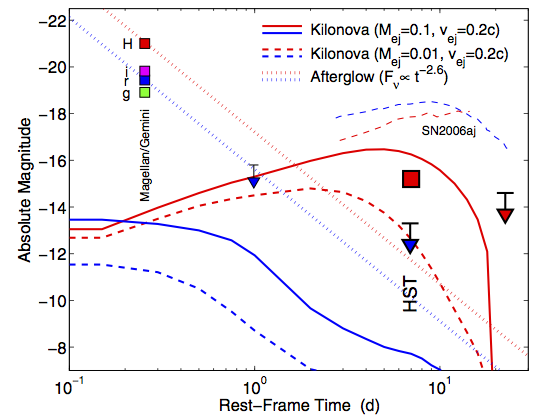
\includegraphics[scale=0.85]{figs/transients/kilonovaBerger.png}
\caption{Kilonova signature in the short GRB\,130603B as revealed by the
Hubble Space Telescope (HST). The Magellan and Gemini telescopes sampled
the optical afterglow of the GRB (dotted lines). The kilonova light
starts to dominate the emission in the H band around a few days after
the merger. Thick and dashed lines: theoretical kilonova models from
\citet{Barnes13} showing that kilonovae are fast-evolving, faint and red
transients. The light-curve of the SN\,2006aj associated with the long
GRB\,060218  is also shown for comparison. From \citet{Berger13}.}
\label{Fig:kilonova}
\end{figure}


% --------------------------------------------------------------------

\subsection{OpSim Analysis and Discussion}
\label{sec:\secname:analysis}

Effective follow up of GW triggers relies on the capability to sample a
relatively large portion of the sky, repeatedly, over a time scale $<1$
week, with different filters \citep{Cowperthwaite15}. In the optical
band, the kilonova signature is expected to be more prominent in the
$i$, $z$  and $y$ filters, which we identify as the most promising
filters for the kilonova search. We emphasize however that another set
of contemporaneous observations in  a ``bluer" filter is necessary to
acquire color information and distinguish kilonovae from other
fast-evolving transients.

We use the median inter-night gap  for visits in the same filter derived
from the candidate Baseline Cadence \texttt{minion\_1016} to show that,
in the absence of a Target of Opportunity (ToO) capability, it is
\emph{not} possible for LSST  to play a major role in the identification
of EM counterparts of GW triggers.

To identify kilonova candidates we need at least 2 observations acquired
within $\sim 1$ week  of the GW event \citep{Cowperthwaite15}. Using the
inter-night gap distribution for visits in the $y$ filter (which is the
most promising filter for a kilonova search), the area of the sky
covered with cadence  $\Delta t<7$ days at any given time, is
$A_{sky}\sim 3000$ deg$^2$ (including deep drilling fields).  This is
the area that can be searched for fast evolving transients.  Two
important considerations follow:

\begin{itemize}
\item[(1)] $A_{sky}$ only covers $P\sim7$\% of the sky. The  probability
that the \emph{entire} GW localization region is contained, by chance,
within $A_{sky}$ is thus very small.
\item[(2)] Even if LSST is able to cover a meaningful portion of the GW
region, we would still not have color information, and we would thus be
unable to filter out contaminating transients.
\end{itemize}

\textbf{We conclude that relying on the serendipitous alignment of the
LSST fields with the GW localization map is not an effective strategy to
follow up GW triggers and identify their EM counterparts. We thus
strongly recommend a ToO capability as part of the baseline LSST
operations strategy.}

Ideally, the ToO capability will allow for imaging of the GW
localization map at least twice over $\Delta t\lesssim$1 week with a
``red" filter ($i$, $z$  or $y$),  and  will include the possibility to
designate a desired set of filters to obtain color information. By the
time of LSST operation the typical size of the GW localization region is
expected to be 10-100 deg$^2$, which would require a small number of
LSST re-pointings. We thus do \emph{not} anticipate a significantly
disruptive impact on other LSST campaigns (especially if only the GW
triggers with the best localizations in the southern sky are selected
for LSST ToOs).

\textbf{At the price of re-shuffling a reasonably small number of
fields, \emph{if} equipped with ToO capabilities, LSST can be the
premier player in the era of EM follow up to GW sources.}

% ====================================================================
%
% \subsection{Conclusions}
%
% Here we answer the ten questions posed in
% \autoref{sec:intro:evaluation:caseConclusions}:
%
% \begin{description}
%
% \item[Q1:] {\it Does the science case place any constraints on the
% tradeoff between the sky coverage and coadded depth? For example, should
% the sky coverage be maximized (to $\sim$30,000 deg$^2$, as e.g., in
% Pan-STARRS) or the number of detected galaxies (the current baseline but
% with 18,000 deg$^2$)?}
%
% \item[A1:] ...
%
% \item[Q2:] {\it Does the science case place any constraints on the
% tradeoff between uniformity of sampling and frequency of  sampling? For
% example, a rolling cadence can provide enhanced sample rates over a part
% of the survey or the entire survey for a designated time at the cost of
% reduced sample rate the rest of the time (while maintaining the nominal
% total visit counts).}
%
% \item[A2:] ...
%
% \item[Q3:] {\it Does the science case place any constraints on the
% tradeoff between the single-visit depth and the number of visits
% (especially in the $u$-band where longer exposures would minimize the
% impact of the readout noise)?}
%
% \item[A3:] ...
%
% \item[Q4:] {\it Does the science case place any constraints on the
% Galactic plane coverage (spatial coverage, temporal sampling, visits per
% band)?}
%
% \item[A4:] ...
%
% \item[Q5:] {\it Does the science case place any constraints on the
% fraction of observing time allocated to each band?}
%
% \item[A5:] ...
%
% \item[Q6:] {\it Does the science case place any constraints on the
% cadence for deep drilling fields?}
%
% \item[A6:] ...
%
% \item[Q7:] {\it Assuming two visits per night, would the science case
% benefit if they are obtained in the same band or not?}
%
% \item[A7:] ...
%
% \item[Q8:] {\it Will the case science benefit from a special cadence
% prescription during commissioning or early in the survey, such as:
% acquiring a full 10-year count of visits for a small area (either in all
% the bands or in a  selected set); a greatly enhanced cadence for a small
% area?}
%
% \item[A8:] ...
%
% \item[Q9:] {\it Does the science case place any constraints on the
% sampling of observing conditions (e.g., seeing, dark sky, airmass),
% possibly as a function of band, etc.?}
%
% \item[A9:] ...
%
% \item[Q10:] {\it Does the case have science drivers that would require
% real-time exposure time optimization to obtain nearly constant
% single-visit limiting depth?}
%
% \item[A10:] ...
%
% \end{description}

% ====================================================================

\navigationbar


% --------------------------------------------------------------------

% ====================================================================
%+
% SECTION:
%    transientFuture.tex
%
% CHAPTER:
%    transients.tex
%
% ELEVATOR PITCH:
%    Ideas for future metric investigation, with quantitaive analysis
%    still pending.
%-
% ====================================================================

\section{Future Work}
\def\secname{\chpname:future}\label{sec:\secname}

In this section we provide a short compendium of science cases that
are either still being developed, or that are deserving of quantitative
MAF analysis at some point in the future.

% ====================================================================

% ====================================================================
%+
% SECTION:
%    sn.tex  
%
% CHAPTER:
%    transients.tex  
%
% ELEVATOR PITCH:
%    Explain in a few sentences what the relevant discovery or
%    measurement is going to be discussed, and what will be important
%    about it. This is for the browsing reader to get a quick feel
%    for what this section is about.
%
% COMMENTS:
% ====================================================================
%+
% SECTION:
%    sn.tex  
%
% CHAPTER:
%    transients.tex  
%
% ELEVATOR PITCH:
%    Explain in a few sentences what the relevant discovery or
%    measurement is going to be discussed, and what will be important
%    about it. This is for the browsing reader to get a quick feel
%    for what this section is about.
%
% COMMENTS:
%
%
% BUGS:
%
%
% AUTHORS:
%  Stefano Valenti , Federica Bianco (@fedhere)
%
% ====================================================================

\section{Young Transients Discrimination Power}
\def\secname{transientsAge}\label{sec:\secname} % For example, replace "keyword" with "lenstimedelays"

\credit{svalenti} % (Writing team)

In this section we investigate the possibility to identify young transients using the intra-night visits. The Baseline Cadence predicts that on average, fields in the main survey get revisited about every 3 days using all filters, and every 15 days when using only r band visits (see section 2.2).  This means that we are likely to discover transients that are between 0 and 3 days old. As pointed out in section 6.1.2, the first hours after the explosion reveal fundamental information on the nature of transients. It is then important to be able to select, among the large number of transients discovered by LSST, the youngest objects. The Baseline Cadence predicts that the second intra-night visit will occur between 30 minutes to 2 hours after the first visit.  The question we are trying to answer here is: Which intra-night gap will maximize the identification of young objects?
To answer this question, we have selected a set of transients with good photometric coverage in the first week after the the outburst/explosion (see left panel of Figure 1) and compute the light curve slope (mag/day) as a function of time (see right panel of Figure 1). In Figure 2,  we report the change in brightness between the first and the second visit for a set of different transients as function of phase from explosion. Despite the heterogeneity in light curves shapes most of the transients show a similar change in brightens on a short time scale. 
This confirms that early classification and identification of interesting transients in a short time scale is a major challenge. However, independently on the type of transient, young transients may be easier to identify with large time gap between visits (2 hours). In general, most of the transients have a large increase in brightness at early phase. 
If the second visit occurs only 30 minutes after the first visit, the change in brightness will be of the order of 1$\%$ or less independently on the type of transient or the time from the start of the outburst/explosion, (see left panel of Figure 2). If the second visit occurs 2 hours after the first visit, the change of brightness will be large enough to be detected for young transients ($\sim$ 5$\%$). 
It is also worth to notice that a larger gap (24 hours), while could help in identify young transients, does not help in identify the type of transient.  The identification of interesting transients, at early stage, can be achieved using supplementary information like historical information from previous visits or color information of the transients.
Finally, we want to stress that the quality of early multiwavelengh data available today is still limited; the sample of astronomical transients used here is not comprehensive and an uniform set of homogeneous data of different transients is still needed in order to further investigate the need of color information. 

\begin{figure}[hbt]
\centerline{
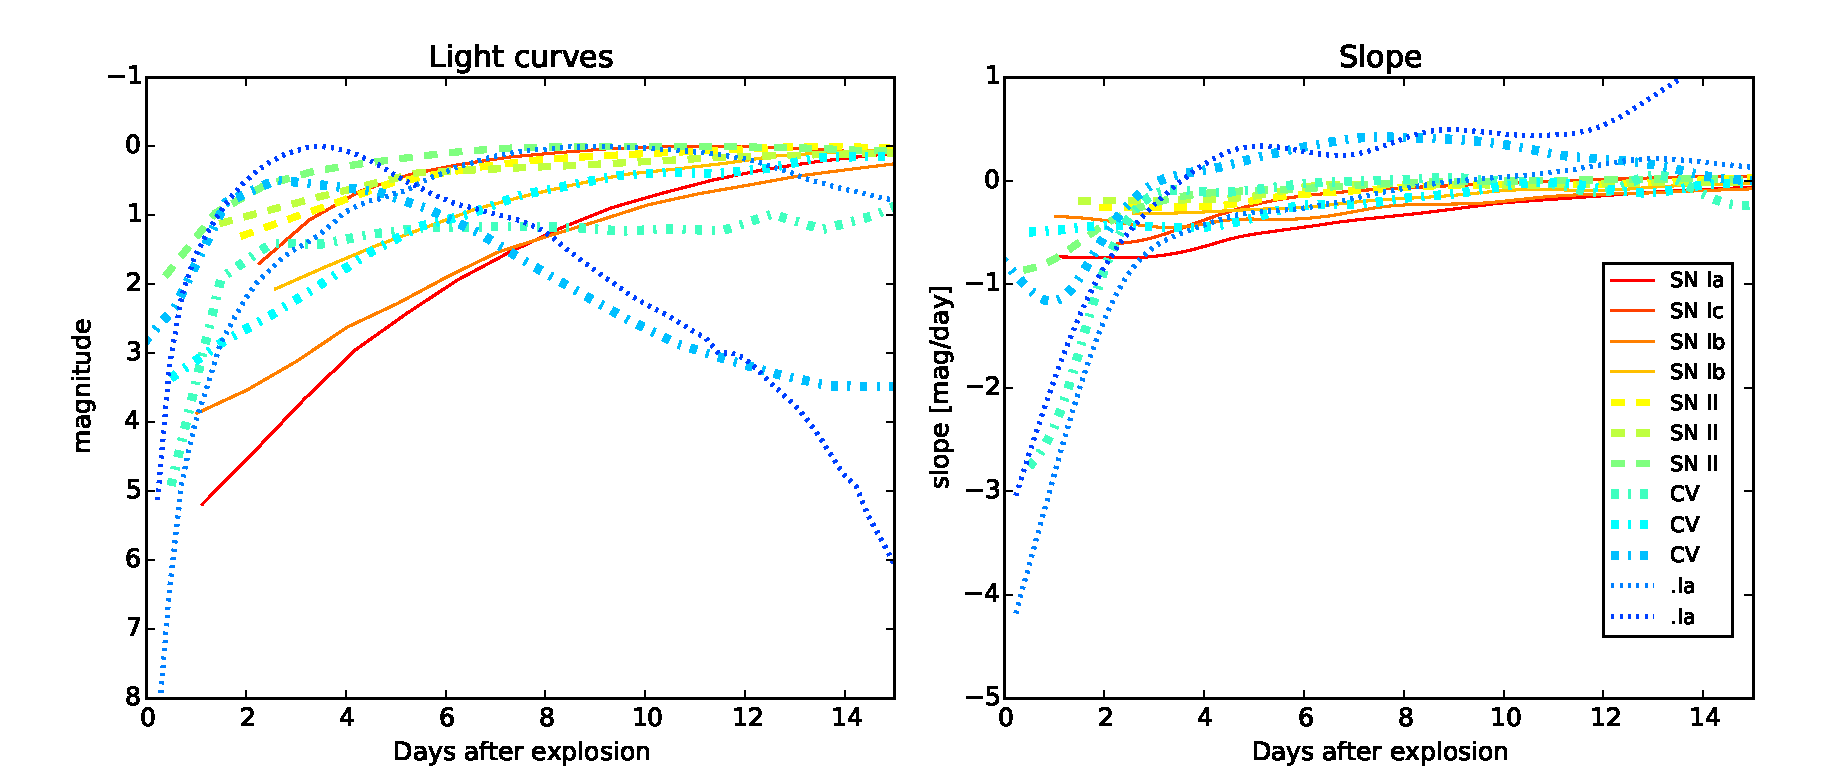
\includegraphics[width=0.6\textwidth]{figs/transients/earlyslope.pdf}
}
\caption{light curve slope [mag/days] of different type of transients as function of the phase from transient outburst/explosion.}
\label{fig:earlyslope}
\end{figure}

\begin{figure}[hbt]
\centerline{
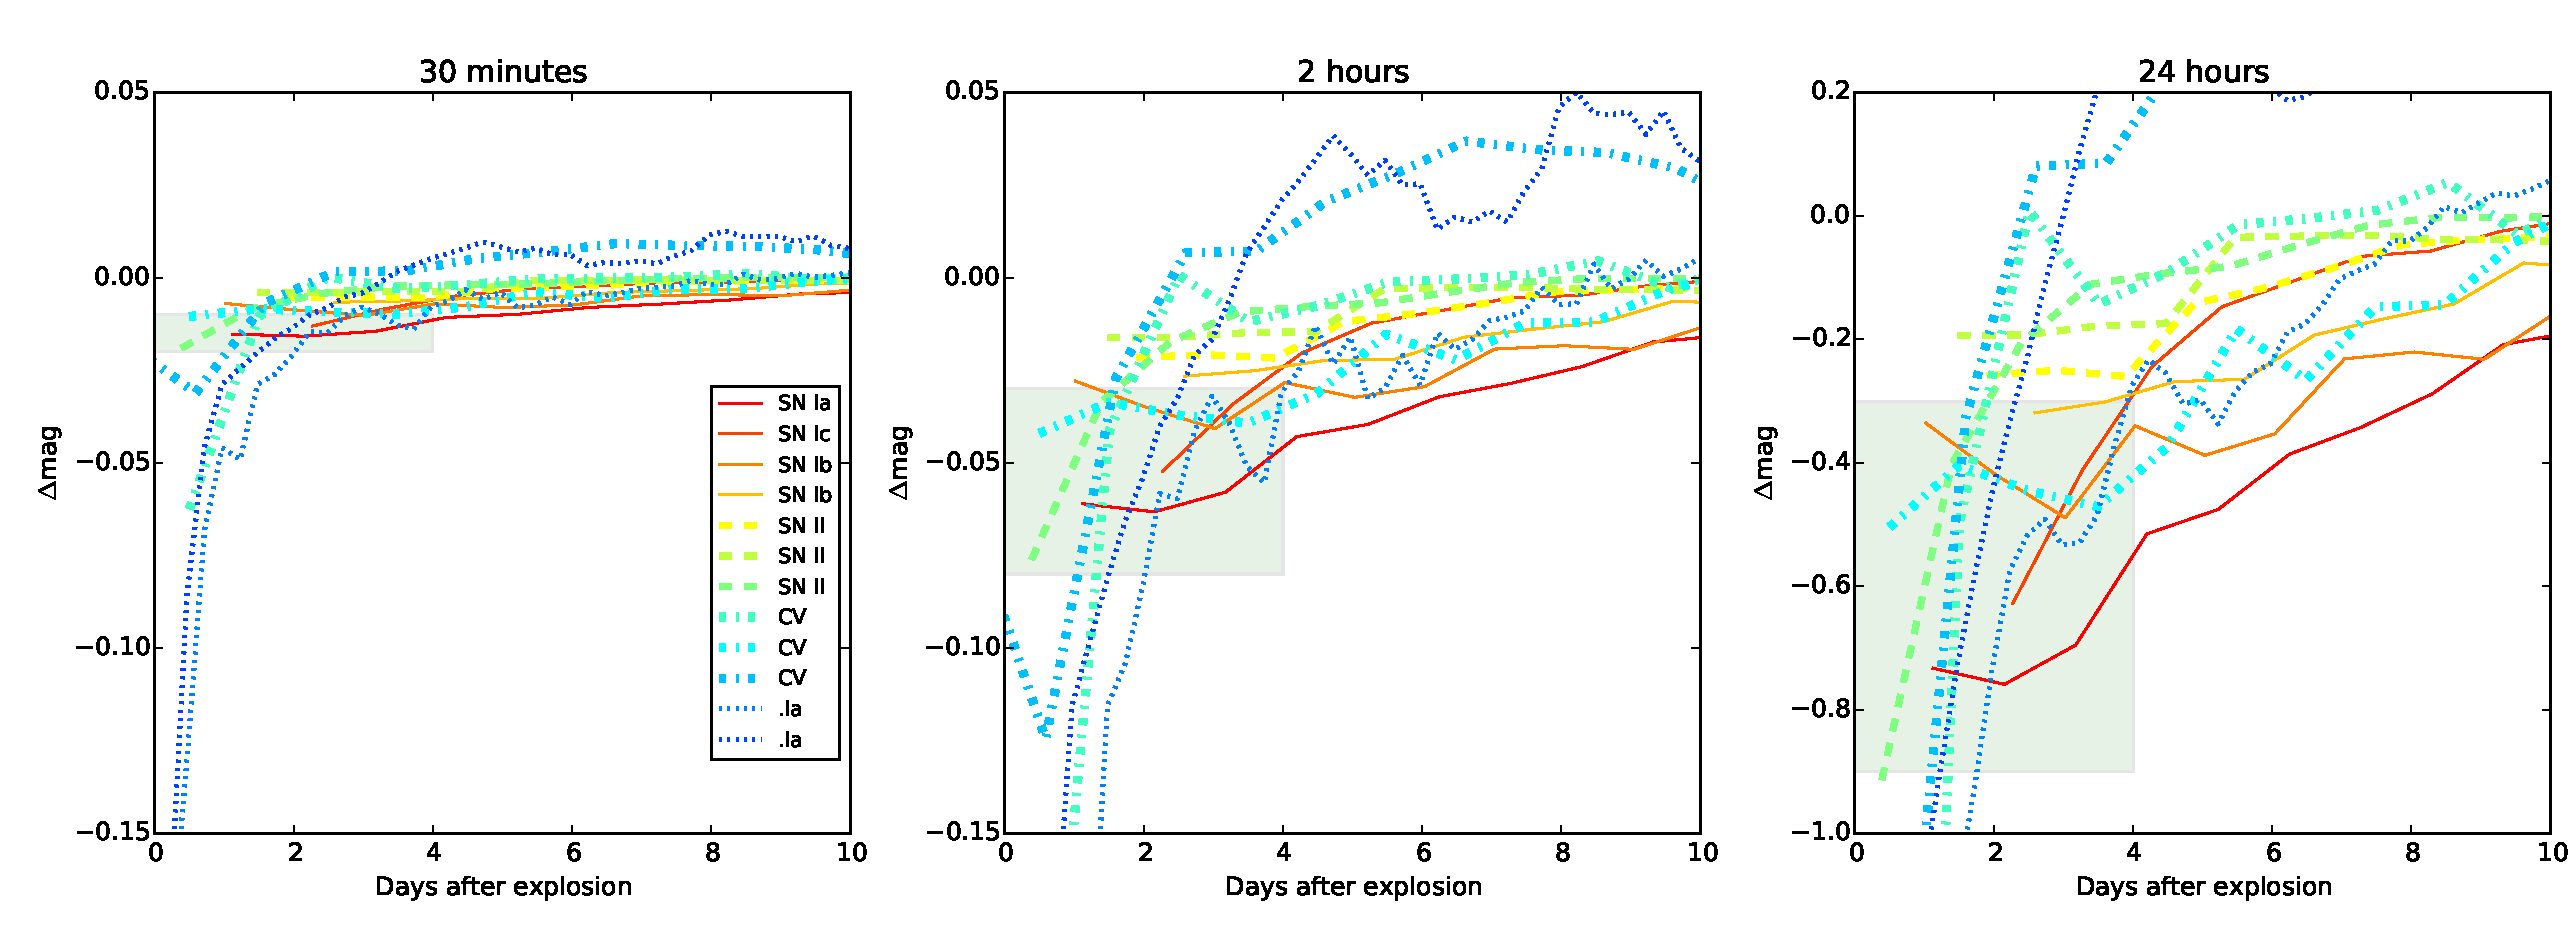
\includegraphics[width=0.6\textwidth]{figs/transients/earlyrise.pdf}
}
\caption{Expected difference magnitudes between two consecutive observations for a set of astronomical transients as a function of the phase of the transient. We consider the cases of the second observation occurring 30 minutes (left panel), 2 hours (central panel) and 24 hours (right panel) after the first observation. Data from: SN~Ia,  Olling et al 2015; SNII, Rubin et al 2016; SN~.Ia, 2010ApJ...715..767S; SN~Ib, Valenti et al 2011, Chao et al 2013; SN~Ic, Mazzali et al 2002; cv, Sokoloski et al. 2013, Finzell, et al in prep .
}
\label{fig:earlyrise}
\end{figure}
%%%%%%%%%%%%%%%%%%%%%%%%
%    Ineed to add the references
%
%Olling et al 2015, Nature, 521, 332O
%Rubin et al 2016, 2016ApJ, 820, 33R
%Valenti et al 2011, MNRAS, 416, 3138V
%Chao et al 2013,  ApJ, 775, 7C
%Mazzali et al, 2002, ApJ, 572L, 61M
%Sokoloski et al. 2013, 2013ApJ...770L..33S
%Finzell, et al in prep



% ====================================================================

% ====================================================================
%+
% SECTION:
%    tde.tex
%
% CHAPTER:
%    transients.tex
%
% ELEVATOR PITCH:
%    Tidal disruption events (TDEs) are the disruptions of stars by supermassive black holes.
%    They can produce flares in the optical and UV (sometimes accompanied by X-ray and radio emission as well).
%    These flares can be used to reveal the properties of otherwise quiescent SMBHs and to study accretion physics.
%    TDEs are rare, LSST will allow the first statistical sample of such events.
%
% AUTHORS:
%    Iair Arcavi (@arcavi)
%
% ====================================================================

% \section{Tidal Disruption Events}
\subsection{Tidal Disruption Events}
\def\secname{\chpname:tdes}\label{sec:\secname}

\credit{arcavi}

A star passing close to a supermassive black hole (SMBH;
$M\gtrsim10^{6}M_{\odot}$) will be torn apart by tidal forces. For
certain ($\lesssim10^{8}M_{\odot}$) black hole masses, the disruption
will occur outside the event horizon and will be accompanied by an
observable flare \citep{Hills1975, Rees1988}. Such flares can be used to
study inactive SMBHs, which are otherwise inaccessible beyond the nearby
($\lesssim100$ Mpc) universe.

We are now building our understanding of how observational properties of
TDEs are affected by the SMBH. Theory claims to provide such a
connection \citep[e.g.][]{Lodato2009, Guillochon2014}, but uncertainties
in the physics of the disruption, subsequent accretion and emission
mechanisms are currently topics of debate \citep[e.g.][]{Strubbe2015,
Guillochon2014, Roth2015}, and new models are vigorously being developed
\citep[e.g.][]{Piran2015, Hayasaki2015, Svirski2015, Bonnerot2015}.

TDEs are rare ($\sim10^{-5}-10^{-4}$ events per galaxy per year;
\citealp{Wang2004, Stone2015}), and until recently, TDE candidates were
discovered mostly in archival data \citep[e.g.][]{Donley2002,
Gezari2006, Esquej2007}. Now, however, wide-field transient surveys have
started discovering TDEs in real time.

Generally, two types of TDE candidates have been identified:
\begin{enumerate}
\item High energy TDEs - The prototype of which is Swift J1644
\citep{Bloom2011, Burrows2011, Levan2011, Zauderer2011}, with two other
events known \citep{Cenko2012, Brown2015}. These events display emission
in $\gamma$-rays and X-rays as well as in the radio, but are not
detected in the optical.
\item Optical-UV TDEs - The prototype of which is PS1-10jh
\citep{Gezari2012}. About $8$ other events are known
\citep{Chornock2014, Arcavi2014, Holoien2014, Holoien2015, Holoien2016}.
Some events were detected also in the X-rays and radio (in addition to
the optical and UV), but the X-ray and radio signatures are different
than those of the high energy TDE candidates.
\end{enumerate}

It is still not clear whether both of these classes of transients are TDEs,
and if so, why they are so different form each other. One option raised is
that some TDEs may launch jets, which when directed towards us, appear as
the high energy events, but otherwise appear as the optical-UV events.
It is still not clear if this is indeed the case \citep[e.g.][]{VanVelzen2013}.

Here we focus on the second type of TDE candidates, which is the
relevant class for LSST, since they can be discovered in the optical.
However, multi-wavelength coordinated observations of
optically-discovered events are required in order to better understand
the connection between the two types of candidates.

The first well-sampled TDE of the optical+UV class was PS1-10jh (discovered by Pan-STARRS;
\citealt{Gezari2012}). \citet{Arcavi2014} later presented three new TDE candidates
from PTF and one discovered by ASAS-SN, all with similar properties
as PS1-10jh. These events exhibit blue colors, broad light curves,
peak absolute magnitudes of $\sim-20$ and a $\sim t^{-5/3}$ decay
at late times. This decay law has been suggested as a unique signature
of accretion-powered TDE light curves \citep{Rees1988, Evans1989, Phinney1989}.
Early-time deviations from the $t^{-5/3}$ rate
can be used to constrain the density profile of the disrupted star
\citep{Lodato2009, Gezari2012}. Late-time deviations would
test the accretion power-source hypothesis altogether.

The spectral signatures of these TDEs are still a puzzle. PS1-10jh displayed
only He II emission lines, lacking any signs of H. Some of the \citet{Arcavi2014}
sample, however, do display H emission.
In fact, a continuum of H / He emission ratios for this class of transients
is being revealed, and is now a focus of theoretical modelling \citep{Strubbe2015, Roth2015}.

The second recent discovery relating to this new sample concerns their
host galaxies \citep{Arcavi2014, French2016}, most of which are
post-starburst galaxies. These galaxies show little or no signs of on-going star formation, but their significant A stellar populations indicate that star formation ceased abruptly a few hundred Myr to a Gyr ago \citep{Dressler1983}. Galaxies with these characteristics often show signs of recent galaxy-galaxy mergers \citep{Zabludoff1996}, which produced the starburst and evolved the bulge. Optical-UV TDEs are intrinsically over abundant in post-starburst galaxies by a factor of $\sim30-200$ (depending on the characteristics of the galaxy; \citealt{French2016}). The reason for the strong preference of TDEs for post-starburst galaxies has still not been determined.

LSST's contribution to TDE studies will be substantial.
\citet{VanVelzen2011} estimate that LSST could discover approximately
4000 TDEs per year. The main drivers for studying TDEs with LSST are:
\begin{itemize}
\item Measuring black hole masses: This involves fitting models to TDE
light curves. It is also relevant to correlate these measurements with
host galaxy properties (mass, bulge/disk decomposition).
\item Constraining galactic dynamics by measuring the TDE rates as
functions of black hole mass and galaxy types.
\item Characterizing TDE emission signatures.
\end{itemize}

A metric is required for measuring how well TDEs can be identified and
distinguished from supernovae and active galactic nuclei. In general, we
expect TDEs to:
\begin{itemize}
\item Be located in the center of their host.
\item Display approximately constant blue (few $10^4$K) colors.
\item Evolve slowly (weeks-months).
\item Not show past AGN-like variability.
\item Preferentially peak around mag -20.
\item Preferentially be hosted in a post-starburst galaxy.
\end{itemize}
These criteria are based on our current knowledge of optical TDEs, which
is still in its early stages. The field is rapidly evolving, and it is
possible that new observations will change the current picture of TDE
emission. This metric is probably best combined with those discussed in
 \autoref{sec:\chpname:SNtransients} for identifying supernovae, though the
luminosity function of TDEs (or what constitutes a ``typical'' TDE light
curve) is not yet known.

A second metric is required to asses the accuracy with which the black
hole mass can be constrained from the TDE light curves. This metric can
be based on existing theoretical models to fit simulated TDE light
curves (such as TDEFit; \citealt{Guillochon2014}).


% ====================================================================

% ====================================================================
%+
% SECTION:
%    sn.tex  
%
% CHAPTER:
%    transients.tex  
%
% ELEVATOR PITCH:
%    Explain in a few sentences what the relevant discovery or
%    measurement is going to be discussed, and what will be important
%    about it. This is for the browsing reader to get a quick feel
%    for what this section is about.
%
% COMMENTS:
%
%
% BUGS:
%
%
% AUTHORS:
%   Federica Bianco (@fedhere)
%
% ====================================================================

\section{Cataclismic Variables}
\def\secname{CVtransients}\label{sec:\secname} % For example, replace "keyword" with "lenstimedelays"

\credit{paulaszkody}, \credit{fedhere} % (Writing team)

Cataclysmic Variables (CVs) encompass a broad group of objects
including novae, dwarf novae, novalikes, and AM CVn systems, all with different
amplitudes and rate of variability. The one thing they all have in
common is active mass transfer from a late type companion to a
white dwarf. The variability ranges from minutes (due to the flickering in
dwarf novae and novalikes, the pulsations in accreting white dwarfs in
the instability strip, or the orbital periods of AM CVn systems), to
hours (for the orbital periods of novae, dwarf novae and novalikes) to
days (for the normal outburst lengths of dwarf novae) to 
weeks (for the outburst length of superoutbursts in short orbital period
dwarf novae and the outburst recurrence time of normal outbursts in short
orbital period dwarf novae) to months (for the outburst recurrence time of 
longer period dwarf novae, various state changes in novalikes and the decline 
in novae) and, finally, to years (for the outburst recurrence timescales of the 
shortest period dwarf novae and the recurrence times in recurrent novae). The 
amplitudes range from tenths of mags for flickering and pulsations to 4 mags 
for normal dwarf novae and changes in novalike states up to 9-15 mags for the 
largest amplitude dwarf novae and regular novae.

These large differences make correct classification with LSST difficult
but necessary in order to reach goals of assessing the correct number
of types of objects for population studies of the end points of
binary evolution. Multiple filters (especially the blue $u$ and $g$) 
along with amplitude and recurrence of variation provide the best
discrimination, as all CVs are bluer during outburst and high states of
accretion. Long term evenly sampled observations can provide indications
of the low amplitude random variability and catch some of the more frequent
outbursts but higher sampling is needed to determine whether an object
has a normal or superoutburst, to catch a rise to outburst or to a
different accretion state or to follow a nova. Novae typically
have rise times of a few days while the decline time and shape provide
information as to the mass, distance and composition. The time to decline
by 2-3 magnitudes is correlated with composition,

***FED: what is a range of time scales for this decline? days? months?

WD mass and location in
the galaxy, thus enabling a study of Galactic chemical evolution.  As with SN, 
the diagnostic power for all these systems rests on color and sampling.   

The metrics rely on a given cadence to provide shape and recurrence time
of large variations that will distinguish between new novae, dwarf novae
outbursts and identify hig vs low states, as well as available blue colors to 
distinguish low amplitude variability that would indicate new pulsators or 
novalikes. The population studies rely on the numbers of long orbital period 
(low amplitude, wide outbursts) vs short orbital period (patterns of short 
outbursts followed by larger, longer superoutbursts) dwarf novae at different 
places in the galaxy, as well as the numbers of recurrent (1-10 yrs) vs normal 
novae (10,000 yrs, about 35/galaxy/yr). Objects particulary worthy of 
discrimination for later followup are the numbers of CVs containing highly 
magnetic white dwarfs. These can be identified by a metric of 10 yrs of data on
a large sample where the magnitude for a majority of the years is a faint (low)
state and a small percentage of time is a bright (high) state, combined with a 
red color (due to cyclotron emission from the magnetic accretion column).


% ====================================================================

% ====================================================================
%+
% SECTION:
%    eruptive.tex
%
% CHAPTER:
%    transients.tex
%
% ELEVATOR PITCH:
%-
% ====================================================================

% \section{LBVs and related non-supernova transients}
\subsection{LBVs and related non-supernova transients}
\def\secname{\chpname:LBVs}\label{sec:\secname}

\credit{nathansmith}

There is a large and diverse class of visible-wavelength transient
sources recognized in nearby galaxies that appear to be distinct from
traditional novae and from SNe, and have often been associated with
the giant eruptions of luminous blue varibles (LBV), such as the 19th
century outburst of $\eta$ Carinae.  Broadly speaking, members of this
class of transients share the common properties that they have peak
luminosities below those of most core-collapse SNe and more luminous
than novae and CVs (absolute magnitudes of roughly $-$9 to $-$15 mag).
They also have H-rich spectra (usually) with relatively narrow lines
that indicate modest bulk outflow velocities of 10$^2$ to 10$^3$ km
s$^{-1}$ (although some have exhibited small amounts of material at
faster speeds).  They tend to evolve on fairly long timescales of
weeks to years (although sometimes they exhibit a quick rise to peak
similar to SNe II-P). This group of transients has gone by many names,
such as LBV eruptions, SN impostors, Type V supernovae,
intermediate-luminosity optical (or red) transients, as well as others
that often include a physical interpretation.  For brevity, these are
often collectively referred to as ``LBVs'', although many of them may
not actually be LBVs.
%This may be largely for historical reasons,
%since LBVs were the first of these to be recognized as a class.  Some
%of the subgroups may be very different from objects like $\eta$
Carinae, however.

Observationally, these eruptions are understood to represent important
and dramatic mass-loss episodes in the lives of massive stars, based
on empirical estimates for the amount of ejected matter.
%Guided
%largely by nearby LBVs with resolved shells, t
These eruptions are
expected to instigate mass loss that is comparable to or more
important than metallicity-dependent winds of massive stars.  This
mode of mass loss, regardless of the mechanism, may be a very
important ingredient in the evolution of massive stars that is
currently not included in stellar evolution models.  Correcting this
is one of the key science drivers in trying to understand the physics
these eruptions.

An important empirical discriminant of subgroups in this class comes
from their progenitor stars.  Some are indeed seen to be very
luminous, blue supergiant stars consistent with traditional LBVs.
Some, however, have somewhat less luminous, heavily dust-obscured
progenitor stars that have been associated with either dust enshrouded
blue or red supergiants, or alternatively, with super-AGB stars of
8-10 M$_{\odot}$, with uncertainty .
%The degeneracy
arises because when the objects are
fully obscured by dust, one cannot actually meaure the star's
temperature, and the bolometric luminosities of super-AGB and red and blue supergiants overlap.  Unfortunately,
cases when we have strong constraints on the quiescent progenitor are
rare, and once they reach their peak luminosity, there is a great deal
of overlap in observed properties.

Theoretically, these eruptions are not understood.  There are many
ideas, but few if any confirmed mechanisms tied to observed
objects.
Some
%previously discussed
theoretical ideas involve (1)
winds driven by super-Eddington instabilities (although the root cause
for suddenly exceeding the Eddington limit remains unexplained), (2)
hydrodynamic explosions caused by deep-seated energy deposition, such
as unsteady nuclear burning, (3) accretion onto companion stars in
binary systems (degenerate or not), (4) mergers in binary and triple
systems, (5) electron-capture SNe, and (6) ``failed SNe'' associated
with a weak explosion and envelope ejection that results from black
hole formation during core collapse.
Because of the relatively low total energy indicated by
radiative luminosities and outflow speeds, these are usually discussed
as non-terminal eruptions, however, the last two are terminal events
that are less luminous and lower energy than normal SNe, and the last
3 should only occur once for a given source.
Together with several well-studied examples that indicate
repeating eruptions, there are indeed many
cases where only one such transient has been seen at the same
position, and some cases where late-time observations suggest that no
source has survived with a luminosity comparable to its progenitor.
%However, there are also several well-studied examples that indicate
%repeating eruptions (multiple repeating transients, multiple nebular
%shells with different ages, etc).
All these theoretical mechanisms
may lead to similar observed phenomena: weak explosions, moderate
luminosities, slow expansion, dusty aftermath, but this class of objects
may represent a mixed-bag of different mechanisms that get lumped
together by default as ``other'' because they are not traditional SNe.

An area of recent interest
is that eruptive non-terminal transients have been observed, in some
cases, to precede much more powerful explosions that are seen as Type
IIn supernovae.  Detectability of SN precursors is discussed in ~\autoref{chp:galaxy}. Even if the pre-SN transients are not observed
directly, pre-SN eruptive mass loss is inferred based on circumstellar
interaction diagnistocs of the SN.  These SN precursors have observed
or inferred properties that are very similar to LBVs and related
transients, 
%.  This may suggest some link between them,
but then again,
most of the LBVs and other SN impostors have been observed for decades
and have not gone SN (yet).  \emph{Being able to distinguish which of these
optical transients are SN precursors and which are not is a major
science driver.}  The amount of mass lost in a precursor eruption may
dramatically alter the type of SN that is observed.  There may also be
a continuum of energies in pre-SN outbursts, extending down to more
normal classes of core-collapse SNe, but these may often go
unrecognized unless the SN is caught very early after explosion.

Rates for these LBV-like eruptions are very poorly constrained,
largely because most previous SN and transient searches with small
telescopes have been optimized for finding more luminous SNe in a
larger volume.  This field begun to change with recent surveys, and will
be revolutionized with LSST.  From discovered examples we have,
numbers are very roughly consistent with a volumetric rate comparable
to that of core-collapse SNe or larger.  %, but with a large error bar.
Rates of individual subclasses are not well constrainted, and limited
information often makes classification into various subgroups
difficult or highly subjective.  The ``rate'' also depends on how
faint the lower limit of inclusions is; evidence suggests that the
brightest events are more rare, and that numbers increase as one moves
to lower luminosity.  At the faint end, it becomes difficult to
distinguish between eruptions and regular variability of LBVs, or
between massive star eruptions and CVs. With deep LSST stacks identifying faint CV in quiescent states this will also change dramatically in the LSST age, with the unvailing of detailed progenitor
information.  Having deep, pre-eruption characterization
of sources at the positions of these eruptive transients (as well as
SN precursors) will likely be a major contribution of LSST.

In terms of timescales, many of the eruptive transients exhibit rise
and decline timescales similar to normal SNe~II-P or II-L, but with
fainter peak luminosity.  For these, observational cadence
requirements will be the same as SNe.  For some eruptive transients,
however, the rise timescales can be very long (rising a few magnitudes
in years).  While LSST's cadence will certainly be fast enough, being
able to discover slowly rising tranients that do not change much from
night to night will be an important metric.

For the faster-rising transients, spectroscopic followup is needed to
discriminate these from normal SNe, and also contextual information
about the host galaxy (and hence, the absolute magnitude) is needed to
differentiate these non-terminal eruptions from Type IIn supernovae
(their spectra look similar, although LBVs do tend to have narrower
lines).  Spectral and color evolution, as well as information about
the progenitor, is needed to distinguish among subgroups within the
class.  Multiwavelength followup is often extremely valuable or even
essential; i.e. mid-IR tells us if an optically invisible source is
cloaked in a dust shell but still quite luminous; Xrays and radio tell
us if an expanding shock wave is the likely source of persistent
luminosity.  For these reasons, nearby cases will continue to be the
most valuable in deciphering the physics of subclasses, whereas the
increased volume in which LSST discovers these fainter transients will
drastically improve our understanding of their rates.  Armed with both
a better understanding of their underlying physics and
characterization, as well as their rates and duty cycles, these
eruptive events can then be incorporated into stellar evolution models
and population synthesis/feedback models.

% % --------------------------------------------------------------------
%
% \subsection{Metrics}
% \label{sec:\secname:metrics}
%
% % --------------------------------------------------------------------
%
% \subsection{OpSim Analysis}
% \label{sec:\secname:analysis}
%
% % --------------------------------------------------------------------
%
% \subsection{Discussion}
% \label{sec:\secname:discussion}
%
% % ====================================================================
%
% \navigationbar


% ====================================================================

